%
% Master thesis template for Ghent University (2018)
%
%
%  !!!!!!!!!!!!!!!!!!!!!!!!!!!!!!!!!!!!!!!!!!!!!!!!!!!!!!!!!!!!
%  !!  MAKE SURE TO SET lualatex OR xelatex AS LATEX ENGINE  !!
%  !!!!!!!!!!!!!!!!!!!!!!!!!!!!!!!!!!!!!!!!!!!!!!!!!!!!!!!!!!!!
%  !! For overleaf:                                          !!
%  !!     1. click gear icon in top right                    !!
%  !!     2. select `lualatex` in "latex engine"             !!
%  !!     3. click "save project settings"                   !!
%  !!                                                        !!
%  !!!!!!!!!!!!!!!!!!!!!!!!!!!!!!!!!!!!!!!!!!!!!!!!!!!!!!!!!!!!
%
%
%  History
%    2014         Doctoral Thesis of Bruno Volckaert
%    2017         Adapted to master thesis by Jerico Moeyersons
%    2018         Cleanup by Merlijn Sebrechts
%
%  Latest version
%    https://github.com/galgalesh/masterproef-template
%
\documentclass[11pt,a4paper,twoside, openany]{book}
\usepackage[a4paper,includeheadfoot,margin=2.50cm]{geometry}

\setlength{\parindent}{0cm}           % indent of the first sentence of a paragraph
\setlength{\parskip}{1em}             % space between paragraphs
\renewcommand{\baselinestretch}{1.2}  % stretch horizontal space between everything

\usepackage{graphicx}
\graphicspath{{images/}}
\usepackage{pdfpages}
\usepackage{enumerate}
\usepackage{float}
\usepackage{caption}
\usepackage{subcaption}
\usepackage[toc,page]{appendix}

\usepackage{minted}                                    % for modern code highlighting
\newenvironment{code}{\captionsetup{type=listing}}{}   % To get multiline code fragments working: https://tex.stackexchange.com/a/53540/72273

\PassOptionsToPackage{hyphens}{url}
\usepackage{hyperref}
\usepackage{url}

\usepackage{quotchap}              % For the fancy quotes next to the chapter titles

\usepackage[numbers]{natbib}       % For bibliography; use numeric citations
\bibliographystyle{IEEEtran}
\usepackage[nottoc]{tocbibind}     % Put Bibliography in ToC

%
% Defines \checkmark to draw a checkmark
%
\usepackage{tikz}
\def\checkmark{\tikz\fill[scale=0.4](0,.35) -- (.25,0) -- (1,.7) -- (.25,.15) -- cycle;}

%
% For tables
%
\usepackage{booktabs}
\usepackage{array}
\usepackage{ragged2e}  % for '\RaggedRight' macro (allows hyphenation)
\newcolumntype{L}[1]{>{\raggedright\let\newline\\\arraybackslash\hspace{0pt}}m{#1}}
\newcolumntype{C}[1]{>{\centering\let\newline\\\arraybackslash\hspace{0pt}}m{#1}}
\newcolumntype{R}[1]{>{\raggedleft\let\newline\\\arraybackslash\hspace{0pt}}m{#1}}

%
% Support for splitting Dutch words correctly
%
\usepackage{polyglossia}
\setdefaultlanguage[babelshorthands=true]{dutch}

% Manually specify additional hypnations for words
\hyphenation{ten-ants appli-caties Open-Stack-Emu cloud-besturings-sys-temen besturings-sys-temen Dev-Stack Volckaert}

%
% Translated strings. If these aren't set, the English words are used.
%
\addto\captionsenglish{%
  \renewcommand{\contentsname}%
    {Inhoudsopgave}%
}
\renewcommand\appendixtocname{Bijlagen}
\renewcommand\appendixpagename{Bijlagen}
\renewcommand{\listoflistingscaption}{Lijst van listings}

% Added by Stijn Brysbaert
% usepackage for markdown
\usepackage[hashEnumerators,smartEllipses]{markdown}
% usepackage for todos
\usepackage[colorinlistoftodos]{todonotes}
\usepackage{verbatim}
% usepackage for glossaries
\usepackage[utf8]{inputenc}
\usepackage[acronym, toc]{glossaries}
% strikethrough
\usepackage{ulem}

\makeglossaries
\newacronym{www}{www}{World Wide Web}

\newacronym{w3c}{W3C}{World Wide Web Consortium}

\newacronym{rdf}{RDF}{Resource Description Framework}

\newacronym{lod}{LOD}{Linked Open Data}

\newacronym{maas}{MaaS}{Mobility as a Service}

\newacronym{uri}{URI}{uniform resource identifier}

\newacronym{id}{ID}{identificator}

\newacronym{eif}{EIF}{European Interoperability Framework}
\makeglossaries
\newglossaryentry{maasaanbieder}
{
    name=MaaS-aanbieder,
    description={Een organisatie die een \acrshort{maas} platform aanbiedt}
}

\newglossaryentry{mobop}{
    name=mobiliteitsoperator,
    plural=mobiliteitsoperatoren,
    description={Een organisatie die van mobiliteit een service maakt en deze aanbiedt aan reizigers}
}

\newglossaryentry{deelmob}{
    name = deelmobiliteit,
    description = {Het delen van een fiets, auto, brommer, ... met andere mensen zodat kosten zoals aankoop en onderhoud kunnen verdeeld worden onder de gebruikers. Kan aangeboden worden als abonnement of pay as you go waarbij voor beide opties de kosten meestal oplopen naar gelang de tijd dat je het voertuig gebruikt}
}

\newglossaryentry{fietsdeelop}{
    name = fietsdeeloperator,
    plural = fietsdeeloperatoren,
    description = {Een combinatie van \gls{mobop} en \gls{deelmob} waarbij het vervoermiddel een fiets is}
}

\newglossaryentry{ontologie}{
    name = vocabularium,
    plural = vocabularia,
    description = {Een vocabularium definieert concepten en relaties (ook termen genoemd) om zaken binnen een bepaalt gebied te omschrijven en weer te geven~\footnote{\url{https://www.w3.org/standards/semanticweb/ontology}}}
}

\newglossaryentry{RDF vocabularium}{
    name = RDF vocabularium,
    description = {Zie \gls{ontologie.}}
}

\newglossaryentry{deeleconomie}{
    name = deeleconomie,
    description = {De deeleconomie is een socio-economisch systeem waarin delen en collectief consumeren centraal staat. Het gaat om gezamenlijk creatie, productie, distributie, handel en consumptie van goederen en diensten\footnote{\url{https://nl.wikipedia.org/wiki/Deeleconomie}}}
}

\newglossaryentry{dock}{
    name = dock,
    plural = docks,
    description = {Een gereserveerde plaats waar exact één voertuig in kan worden geparkeerd. In sommige gevallen is een dock enkel en alleen bruikbaar voor het parkeren van een specifiek vervoermiddel. Voertuigen van een ander type dan waarvoor het dock is bedoeld, kunnnen hier niet worden geparkeerd}
}

% Added by supervisor Pieter Colpaert to make comments
\newcommand{\pc}[1]{\noindent\textcolor{red}{\{Pieter says: #1{\bf \}}}}
%
% Set the title and your name
%
\title{Het publiceren van gegevens rond fietsdeeloperatoren als Linked Data}
\author{Stijn Brysbaert}

%
%  END OF HEADER
%  The actual latex document content starts here.
%
\begin{document}

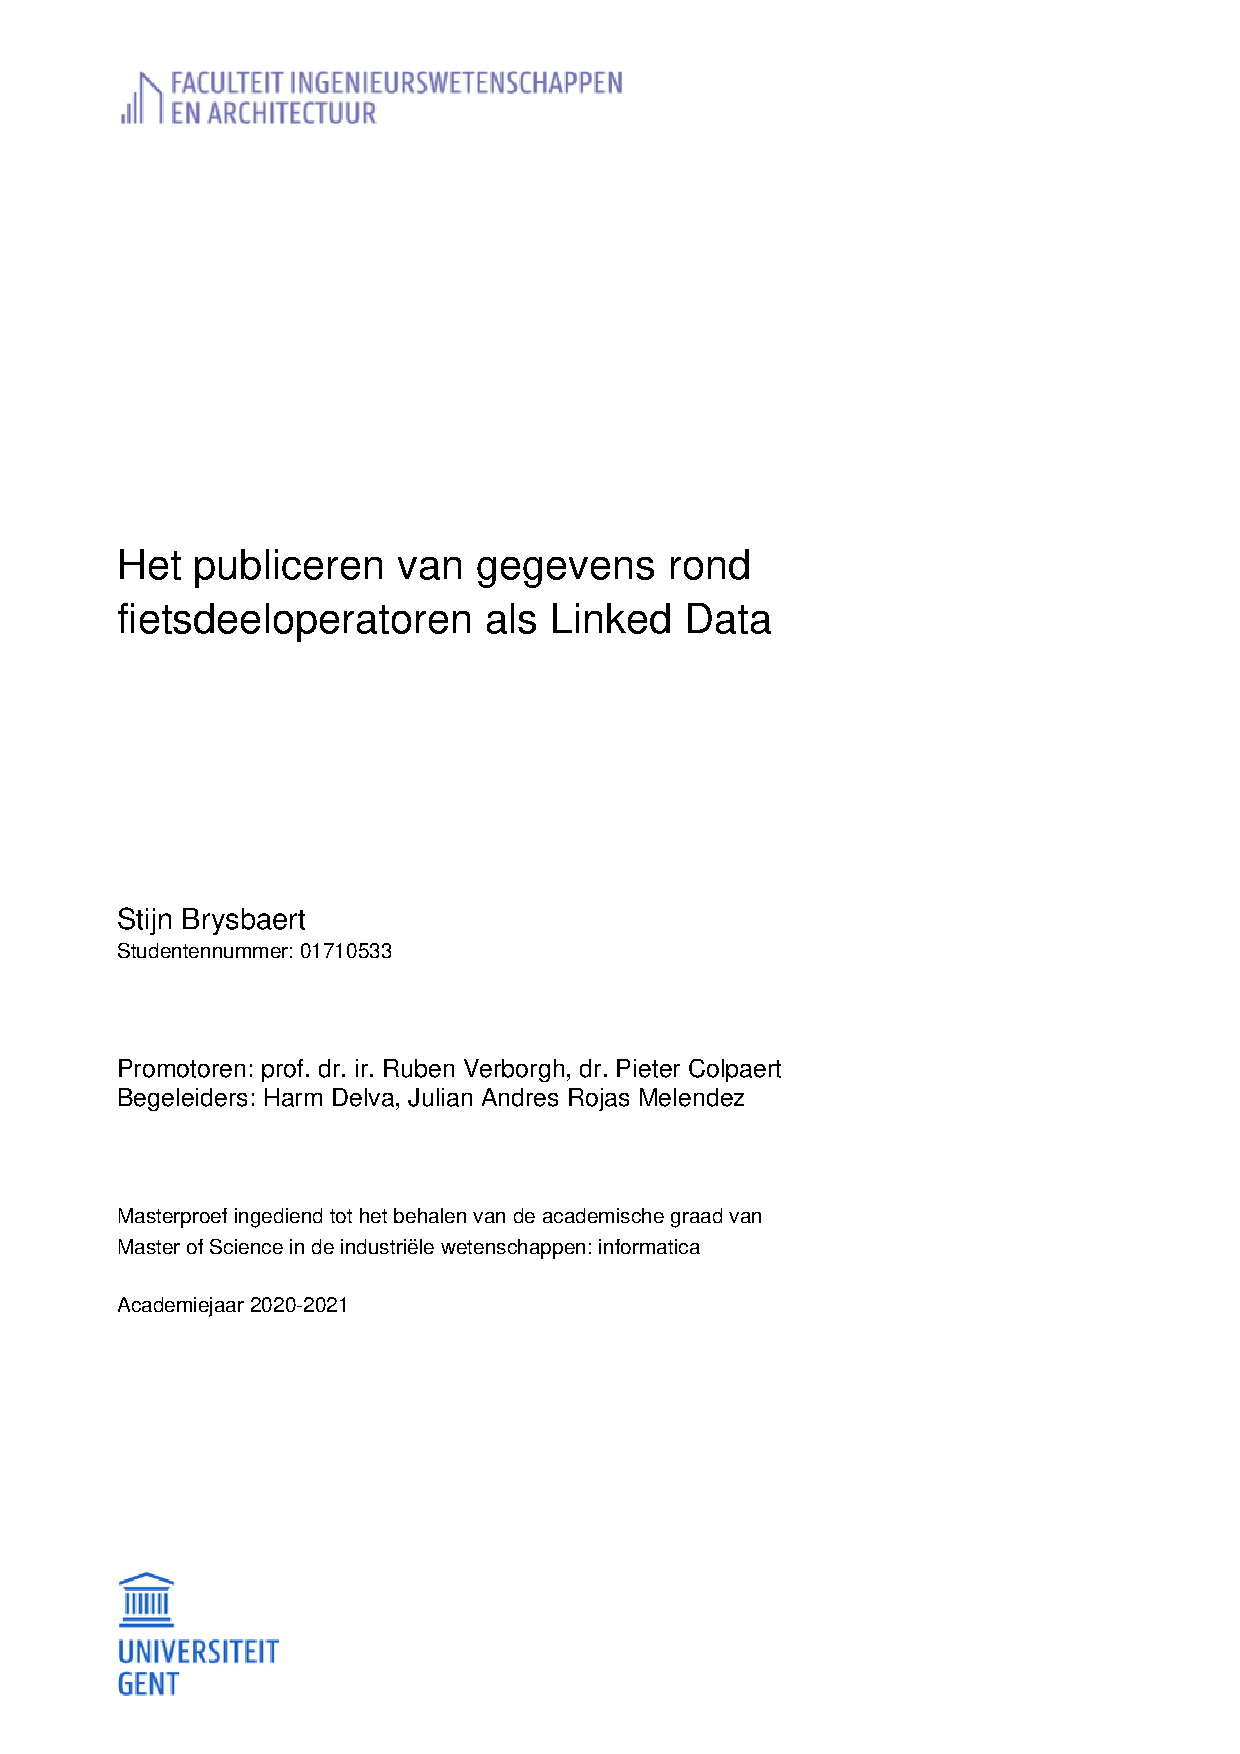
\includepdf{voorblad.pdf}             % Front matter
\newpage\thispagestyle{empty}\mbox{}  % White page
\thispagestyle{empty}    % Don't show page number

\begin{center}
\textbf{Dankwoord}
\end{center}

Deze masterproef is het eindwerk van mijn masteropleiding en daarmee ook het einde van mijn hoger onderwijs traject. Na het behalen van een professionele bachelor startte ik een schakeljaar industriële wetenschappen afstudeerrichting informatica om daar aansluitend de bijhorende masteropleiding af te leggen. Door dit te combineren met de rol als groepsleider van een scoutsgroep met 360 leden werd dit een intensieve periode van drie en een half jaar. Gedurende die periode stond ik er gelukkige nooit alleen voor. Ik kon rekenen op veel mensen rondom mij die me ondersteunden op vlak van zowel scouting als studies. De ruimte dat dit dankwoord mag innemen is helaas te klein om al die namen te vernoemen. Toch had ik graag mijn ouders vermeld en hun bedankt mij de mogelijkheid te geven te kunnen studeren wat, wanneer en hoe ik zelf wilde. Ik ben me ervan bewust dat dit een uitzonderlijke kans is. Dankjewel iedereen.

Deze masterproef kwam tot stand met de onmisbare hulp van een aantal personen. Allereerst had ik mijn promotoren prof. dr. ir. Ruben Verborgh en dr. Pieter Colpaert willen bedanken mij de kans te geven me te kunnen verdiepen in de interessante en veel belovende wereld van Linked Data. Daarbovenop op wil ik Pieter extra bedanken voor zijn enthousiasme en gedrevenheid in het onderwerp. Mijn doel iets interessant te maken van mijn masterproef werd ook zijn doel. Altijd beschikbaar en paraat met kritische ideeën en feedback. Ook mijn begeleiders Brecht Van de Vyvere, Dylan Van Assche, Julian Andres Rojas Melendez en Harm Delva wil ik bedanken voor hun vooral technische ondersteuning via ons mattermost kanaal op ieder moment van de dag. Speciale dank gaat uit naar mijn broer Maarten\footnote{\url{https://www.linkedin.com/in/maarten-brysbaert}} die me op zeer korte tijd een demo hielp in elkaar steken waarmee ik mijn contributies kon visualiseren tijdens presentaties.

Om af te sluiten had ik graag mijn vriendin Feuille Boi bedankt voor haar onvermoeibare steun, ook tijdens moment waarop dat niet zo vanzelfsprekend was. Ook mijn zussen die altijd blij waren me te zien als ik thuis kwam waren een steun. Daarnaast wil ik mijn huisgenoten Aileen Bonne en Wiebe Vermiesch bedanken voor de leuke momenten tussendoor en andere scoutsvrienden voor de ontspannende wandelingen mét social distancing uiteraard. Extra dank gaat uit naar Aileen voor de zelfreflectie momenten ten behoeve van mijn masterproef.

Bedankt allemaal!
\newline
Stijn Brysbaert          % Word of thanks
\newpage\thispagestyle{empty}\mbox{}  % White page
% \listoftodos
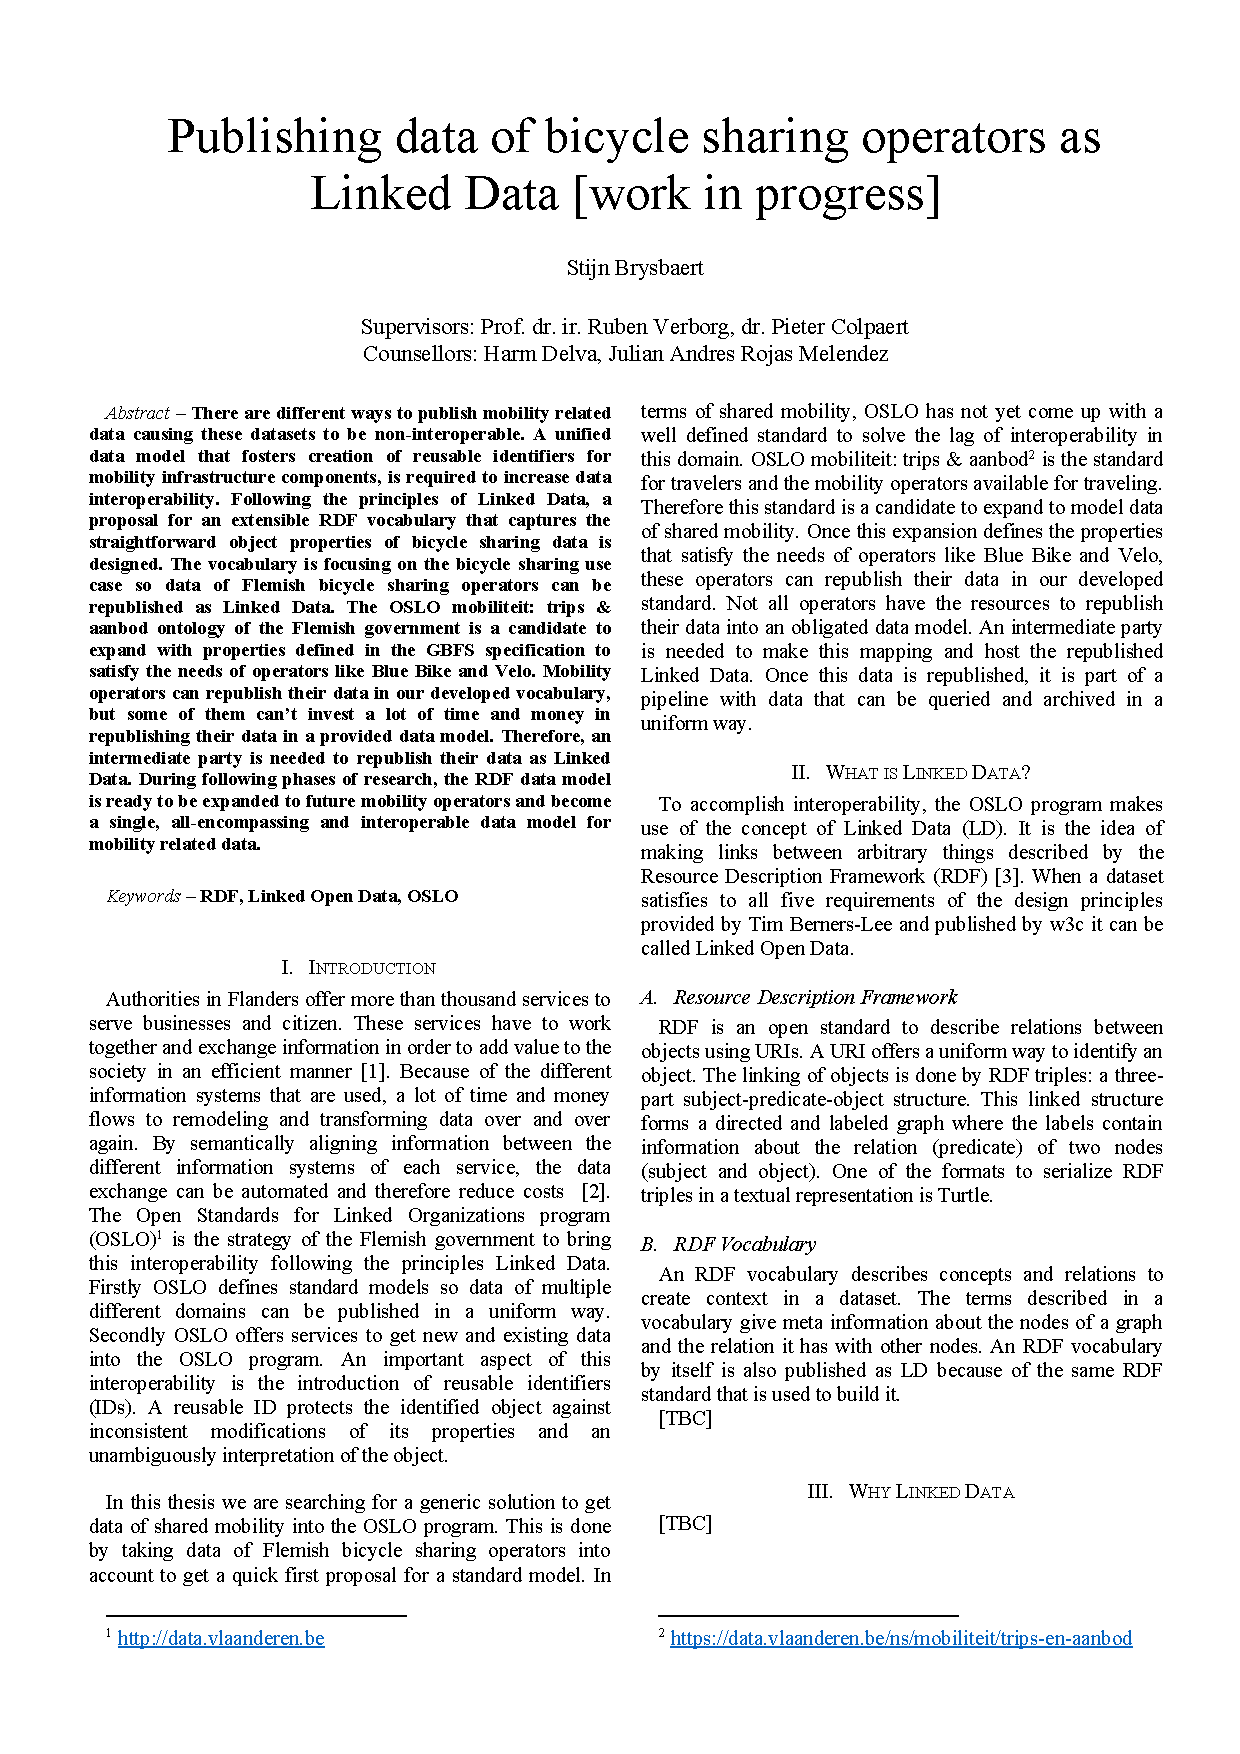
\includepdf[pages={-}]{abstract.pdf}  % Extended Abstract

\tableofcontents                      % Table of Contents
\listoffigures                        % List of figures
\listoftables                         % List of tables
\listoflistings                       % List of listings (code fragments)
\printglossary
\printglossary[type=\acronymtype]

%
% Include the main chapters of the thesis below
%


\chapter{Interoperabiliteit van gegevens}
\label{chap:interoperabele_gegevens}
Wanneer gegevens gemodelleerd worden vanuit één enkel perspectief kunnen ze niet gecombineerd worden met andere informatie bronnen of geïntegreerd worden in andere toepassingen en business processen~\cite{interoperability}. Gegevens uit het ene ICT systeem zullen dus niet zomaar bruikbaar zijn in een ander systeem. Bijvoorbeeld, busmaatschappij De Lijn haalt informatie op over wegenwerken uit de database van het Vlaamse Agentschap Wegen en Verkeer. Die informatie kan nuttig zijn om eventuele wegenwerken die het busverkeer hinderen op te sporen. De Lijn kan op basis van deze informatie aanpassingen aanbrengen in de dienstregeling zodat die buslijn\footnote{Busmaatschappij De Lijn gebruikt de term 'lijn' om een bepaalt traject van A naar B aan te duiden.} bedient blijft. In een niet-interoperabel scenario, zal de busmaatschappij voor ieder resultaat uit de wegenwerken database manueel moeten nagaan of lopende werken één of meerdere lijnen doorkruisen of niet. In een wereld waar gegevens tussen de publieke en private sector wel interoperabel zijn, kunnen de systemen van de ene partij overweg met de gegevens van een andere partij. Het computersysteem van De Lijn zal de resultaten van een query, uitgevoerd op de database van Agentschap Wegen en Verkeer, automatisch kunnen interpreteren en het personeel van De Lijn kunnen waarschuwen voor potentiële hinder op een bepaalt deel van een lijn. Daarna kunnen verdere, eventueel manuele, acties worden ondernomen.

Dankzij interoperabiliteit tussen gegevens krijgen organisaties de mogelijkheid om informatie en kennis te delen op hun eigen manier door middel van gegevensuitwisseling tussen ICT systemen. Het \acrfull{eif} beschrijft een model voor interoperabiliteit dat toepasbaar is op Europese digitale publieke diensten. Met dit programma wilt Europa bouwen aan een naadloze gegevens doorstroming binnen Europese publieke diensten zoals het Vlaams Agentschap voor Wegen en Verkeer in het voorbeeld hierboven~\cite{neweif}. In de volgende secties van dit hoofdstuk wordt er dieper ingegaan op wat die interoperabiliteit precies is en hoe die kan worden geïmplementeerd.

\section{Semantische interoperabiliteit}
\label{sec:semantische_interoperabiliteit}
Semantische interoperabiliteit gaat over de betekenis en relaties tussen gegevens. Het behandelt zowel syntactische als semantische aspecten. Interoperabiliteit verzekert dat het formaat (syntactisch) en de inhoud (semantisch) van informatie dat werd verzonden, bewaart blijft en wordt begrepen door de ontvanger zoals bedoeld door de verzender. Met andere woorden: Wat werd verzonden, is wat werd begrepen~\cite{neweif}.

Het is niet voor de hand liggend dat iets wordt geïnterpreteerd zoals het werd bedoeld. Als de verzender spreekt over het Sint-Pietersplein, kan dit worden geïnterpreteerd als meerdere verschillende plaatsen of objecten. De ene ontvanger denkt hierbij aan het Sint-Pietersplein in Gent, maar iemand anders denkt direct aan het plein in Vaticaanstad. Parking P10 in Gent heeft dezelfde naam, die bevindt zich onder het Sint-Pietersplein in Gent. Dit probleem doet zich ook voor bij gegevens in een database.

Met behulp van metadata kan duidelijk worden gemaakt wat er precies wordt bedoeld met een bepaalt object. Door relaties tussen objecten te omschrijven kan er nog meer context worden gecreëerd waardoor zowel mens als computer beter kan begrijpen wat er wordt bedoeld door de zender. Om relaties tussen objecten mogelijk te maken zijn er herbruikbare identificatoren nodig die een object uniek identificeren.

\section{Herbruikbare identificatoren}
\label{sec:herbruikbare_ids}
De databases van publieke sectoren bevatten miljoenen objecten. Het is mogelijk dat een zelfde object gebruikt wordt door meerdere verschillende partijen. Neem bijvoorbeeld een fietsenstalling aan een busstation waar reizigers hun fiets kunnen plaatsen als ze de bus nemen, maar waar ook deelfietsen van bijvoorbeeld Velo kunnen worden ontleend. In dat geval wordt het gebruik en de verantwoordelijkheid van dat object uitgebreid naar meerdere partijen: meerdere \glspl{mobop} en diensten van de stad/gemeente die bijvoorbeeld in onderhoud en reparaties voorziet. Gezien dat gedeeld gebruik hebben alle partijen toegang nodig tot de gegevenssets waarin de parameters van dat object lees- en schrijfbaar zijn. Zo een situatie vraagt om interoperabiliteit van gegevens en herbruikbare identificatoren die deze objecten aanduiden. 

Neem als voorbeeld de situatie in figuur~\ref{fig:busstation_labels}. Een busmaatschappij gebruikt de \acrfull{id} van een busstation om aan te duiden waar een bepaalde bus zal stoppen. Terwijl de operator achter de Velo fietsen dat \acrshort{id} zal hergebruiken om aan te duiden dat er een fietsenstalling bij dat busstation is te vinden. Als er elektriciteitsvoorzieningen nodig zijn tot bij het object, kunnen elektriciens door middel van het busstation ID en andere technische informatie precies weten hoe ze te werk moeten gaan. Zo kunnen er bijvoorbeeld verlichtings- en oplaadpunten voor elektrische fietsen worden voorzien en informatie hierover gekoppeld worden aan de ID's van het busstation en fietsenstalling.

\begin{figure}[h]
	\centering
	\begin{subfigure}{\textwidth}
		\centering
		\centerline{
			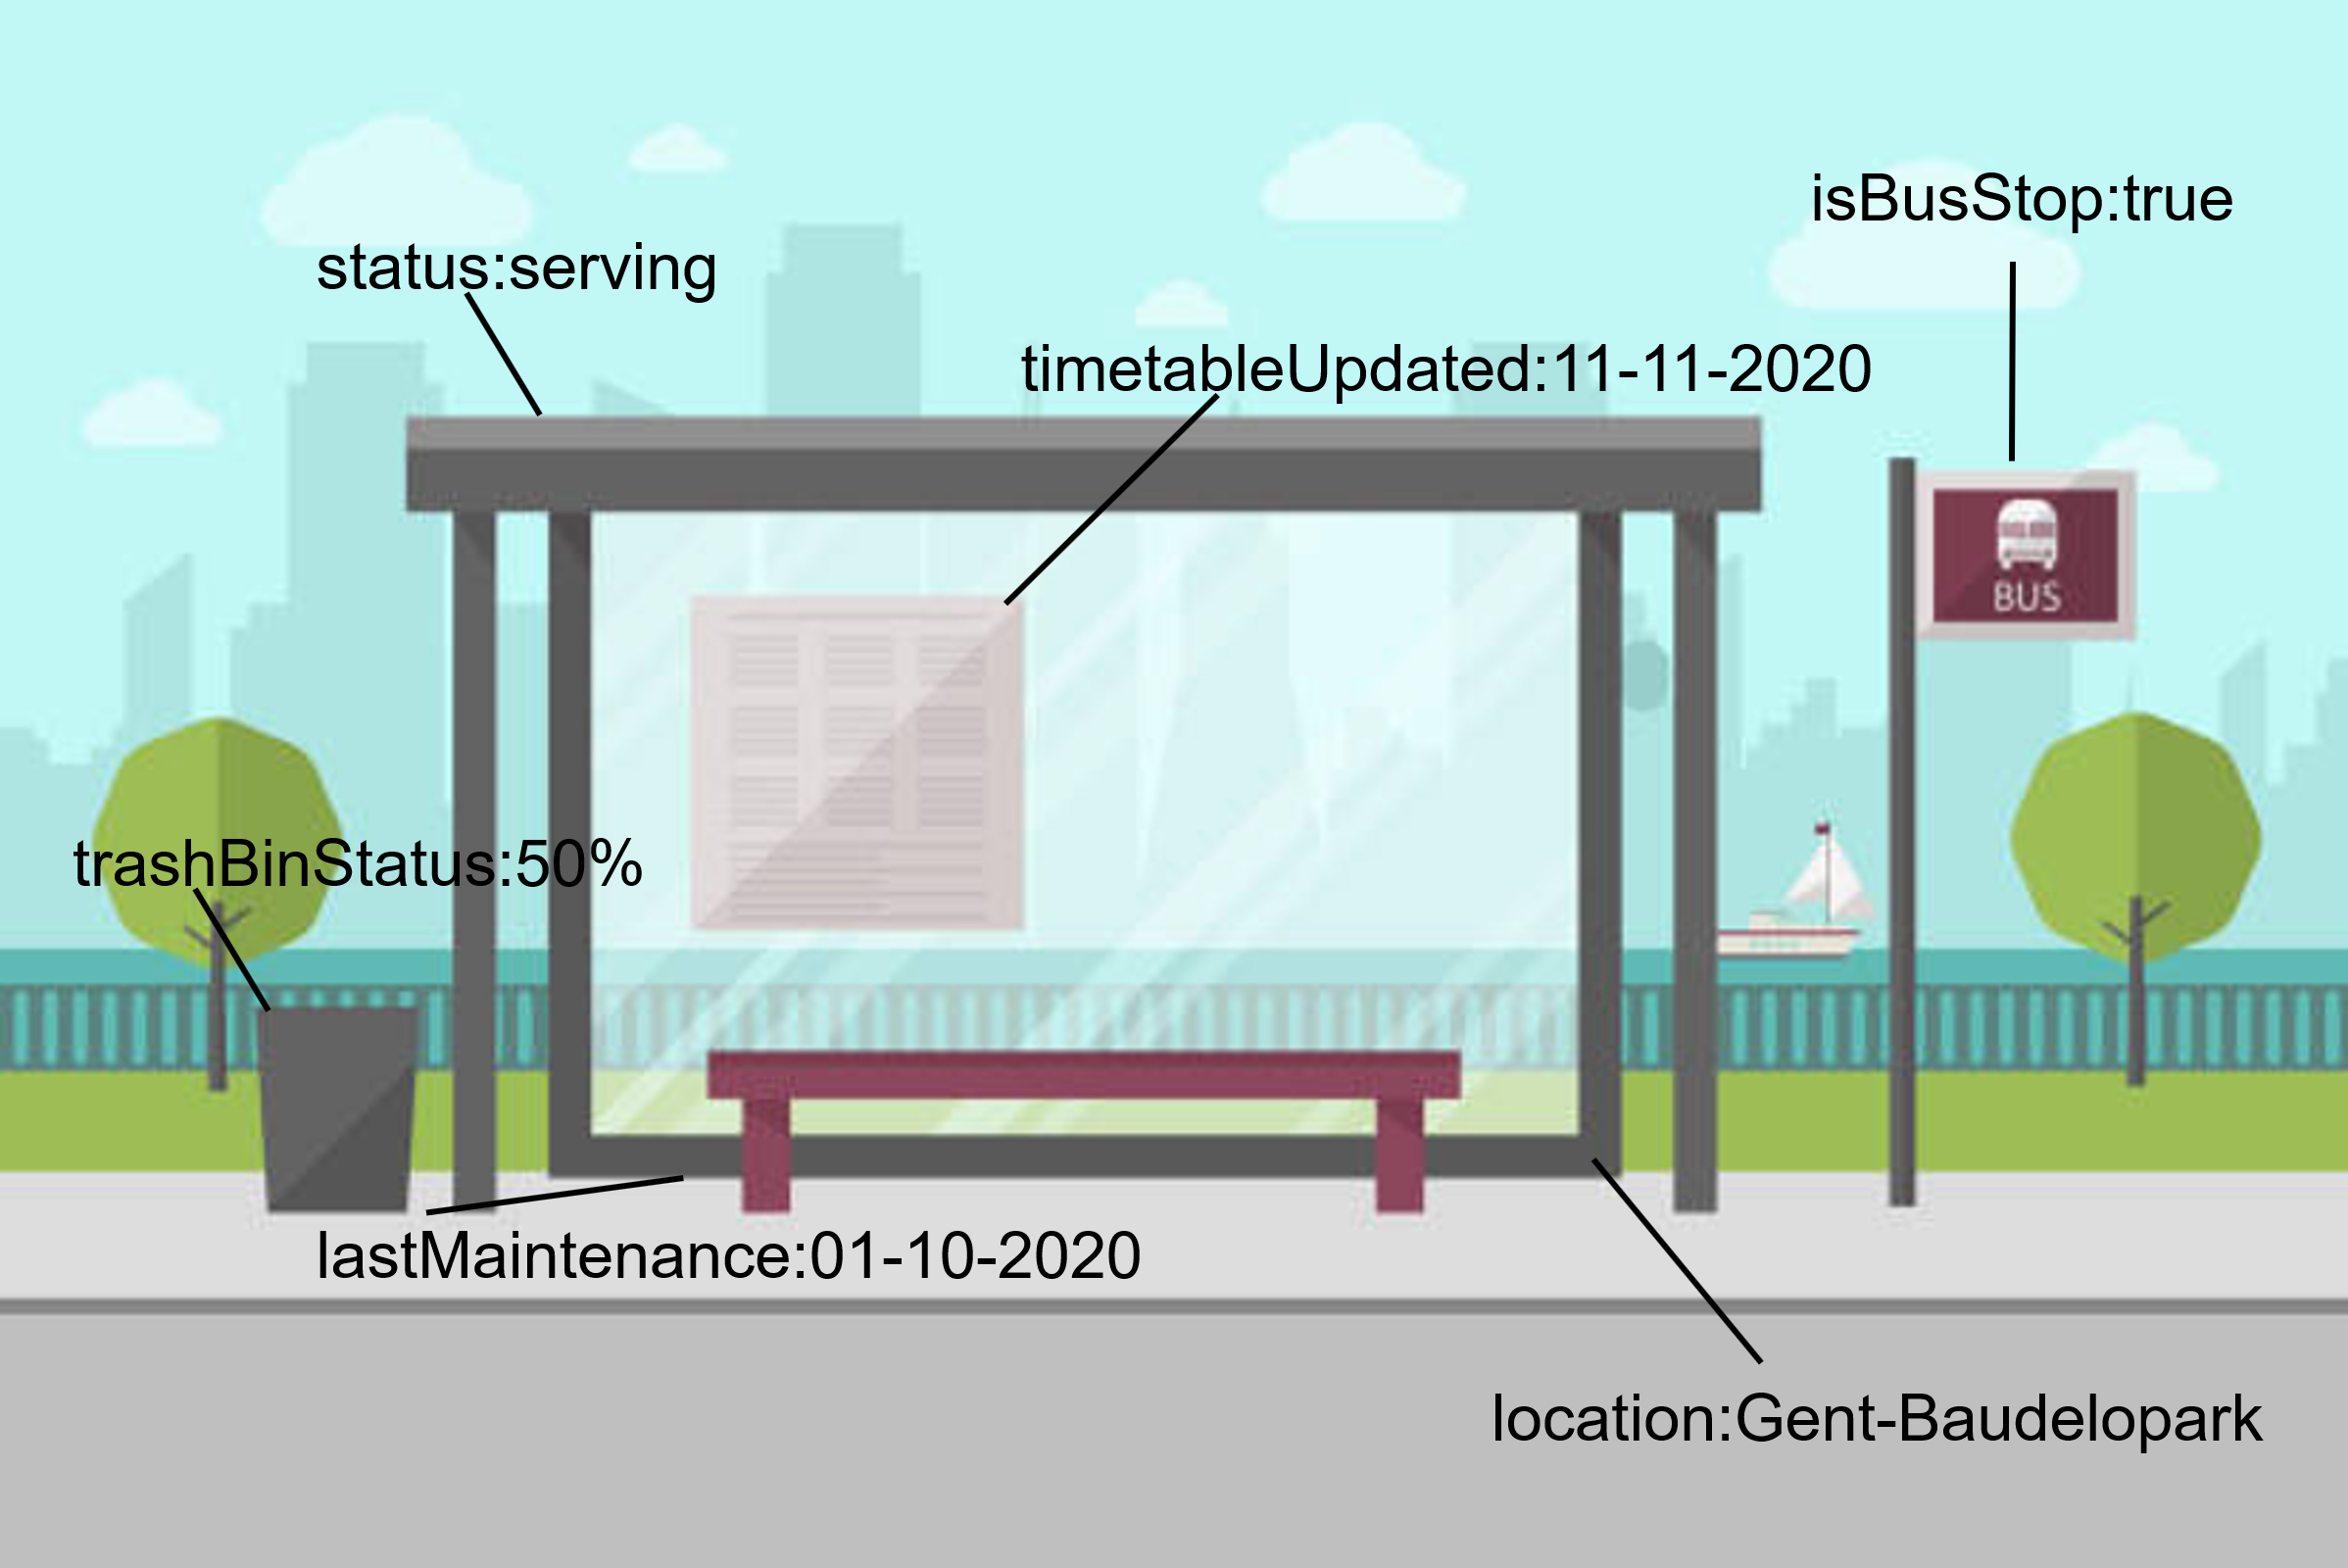
\includegraphics[scale=0.35]{images/busstation_labels.png}
		}
	\end{subfigure}
	\caption{Parameters van een infrastructuur object, gebaseerd op een figuur van istockphoto.com}
	\label{fig:busstation_labels}
\end{figure}

\section{Open Standaarden voor Linkende Organisaties}
\label{sec:OSLO}
Het Vlaams interoperabiliteitsprogramma Open Standaarden voor Linkende Organisaties (OSLO)\footnote{\url{https://data.vlaanderen.be}} is een initiatief van de Vlaamse overheid om hergebruik van gegevens te stimuleren. Het is een van de stappen die Vlaanderen neemt richting een Open Overheid met als doel een nauwere samenwerking te creëren tussen overheid en de privé sector.
Een vorige stap naar open data was het openbaar beschikbaar maken van het Grootschalig Referentiebestand (GRB). Het GRB is een digitale topografische referentiekaart van Vlaanderen waarop alle gebruikers eigen geografische gegevens kunnen aanduiden. Deze locatie gegevens van gebouwen, percelen, wegen en hun inrichting, waterlopen, spoorbanen en het wegennetwerk identificeren miljoenen objecten in Vlaanderen. Dit referentiebestand wordt gebruikt voor onder andere dispatchingtool bij hulpdiensten en het lokaliseren en intekenen van ondergrondse kabels en leidingen~\cite{wat_is_grb}. Sinds het GRB openbaar beschikbaar werd via een gegevensportaal\footnote{\url{http://opendata.vlaanderen.be}} is het gebruik ervan enorm toegenomen~\cite{grb_OD}.

Desondanks de nuttige toepassingen dat het systeem brengt, ondervinden heel wat gebruikers (private partners, bevolking en publieke administratiediensten) moeilijkheden bij het verbinden met en interpreteren van deze open data bronnen. Deze problemen met de interoperabiliteit van gegevens veroorzaken strubbelingen bij het hergebruiken van deze publieke sector informatie~\cite{opengovernment}. Om de vraag naar interoperabele gegevens te beantwoorden werd het OSLO programma opgestart dat verder bouwt op de principes van Linked Data en voldoet aan de aanbevelingen uit het \acrshort{eif}.

Het OSLO programma legt de betekenis vast van concepten, woorden en definities en hoe ze te structureren zijn in databases of softwarepakketten. Dankzij deze afspraken, omschreven in datastandaarden, kunnen semantische discussies en misverstanden worden vermeden~\cite{OSLO_handleiding}.

\subsection{OSLO services}
Informatie Vlaanderen biedt verschillende services aan waarmee het organisaties, in zowel de publieke als privé sector, op het OSLO traject helpt. Samen met de organisatie in kwestie onderzoekt het OSLO-team in hoeverre de aangeleverde informatiemodellen kunnen afgestemd worden op bestaande OSLO vocabularia. Nadat de noden voor een gegevensmodel in kaart gebracht werden, zal het team een datastandaard (of OSLO vocabularium) ontwikkelen volgens `Proces \& Methode' van OSLO\footnote{\url{https://data.vlaanderen.be/cms/Proces_en_methode_voor_de_erkenning_van_datastandaarden_v1.0.pdf}}, dat zijn richtlijnen voor het ontwikkelen van nieuwe standaarden binnen OSLO. Nadat er een gepaste datastandaard ontwikkeld of een reeds bestaande standaard toegewezen werd, wordt er ook ondersteuning geboden bij het implementatieproces.

\section{Verhoogde interoperabiliteit met OSLO}
Het doel van OSLO is om de gegevensoverdracht tussen verschillende organisaties te versnellen en automatiseren. Dit is nodig omdat de overheid meer dan duizend diensten aanbiedt aan burgers en bedrijven~\cite{OSLO_handleiding}. Deze samenwerking kost tijd en geld doordat gegevens niet interoperabel zijn. Dankzij de hulp van de experten binnen Informatie Vlaanderen die OSLO mogelijk maken, wordt de nood aan interoperabele gegevens tegemoetgekomen. Gegevens worden eenduidig gedefinieerd en hergebruikt met als resultaat meer samenhang tussen informatie en bijgevolg betere begrijpbaarheid en vindbaarheid ervan.

De huidige doelstelling bestaat erin om zoveel mogelijk gegevenssets te (her)publiceren als \acrshort{lod} met behulp van het OSLO programma. Gegevens rond nieuwe projecten kunnen vanaf nul worden opgebouwd met gestandaardiseerde gegevensmodellen. Reeds bestaande gegevenssets moeten worden omgevormd, zodat het gebruikmaakt van die standaard modellen. Hiervoor zijn tools nodig die verder in deze scriptie worden besproken.

\chapter{Linked Data}
\label{chap:intro}

Tim Berners-Lee, de grondlegger van het \acrfull{www} en oprichter van het \acrfull{w3c}, pleit al jaren voor ``raw data''\footnote{video:  \url{https://www.ted.com/talks/tim_berners_lee_the_next_web} op 10'40''}. Daarmee vraagt hij aan instellingen zoals overheden, onderzoekscentra en bedrijven om hun gegevens openbaar op het internet beschikbaar te stellen zodat het toegankelijk is voor iedereen om er onderzoek op uit te voeren~\cite{tedtalk}. Het openbaar maken van data en het zo ter te beschikking stellen voor iedereen zou wereldverbeterende inzichten moeten opleveren zoals economische groei, efficiënter gebruik van resources en een beter leefwereld voor burgers~\cite{tedtalka}.

\section{Linked Open Data}
\label{sec:linked_open_data}
Om uit al die beschikbare data op het Web inzichten te kunnen verwerven, is er nood aan hulpmiddelen die gegevens met elkaar in verbinding brengen zoals hyperlinks doen met documenten. Die hulpmiddelen samen vormen een framework, het Semantisch Web genoemd, waarmee gegevens kunnen worden gepuliceerd volgens het vijfsterrenmodel van Tim Berners-Lee. Open data krijgt vijf sterren wanneer het voldoet aan een aantal voorwaarden: de gegevens moeten online beschikbaar zijn in een open bestandsformaat, bovendien moet het gebruikmaken van de w3c\footnote{\url{https://www.w3.org/standards/}} standaarden zoals \acrfull{rdf} en SPARQL zodat anderen naar de dataobjecten kunnen verwijzen. De gegevens zelf moeten ook verwijzen naar gegevens van anderen zodat er meer context kan gecreeërd worden. Gegevens met vijf sterren worden ook wel \acrfull{lod} genoemd~\cite{opendata}.

\begin{figure}
	\centering
	\begin{subfigure}{\textwidth}
		\centering
		\centerline{
			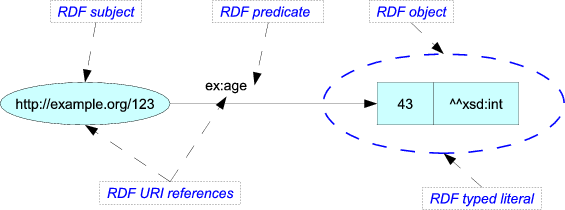
\includegraphics[scale=0.75]{images/rdfexample.png}
		}
	\end{subfigure}
	\caption{Voorbeeld van een \acrshort{rdf} graaf~\cite{rdfgraph_img}}
	\label{fig:rdf_example}
\end{figure}

\section{Resource Description Framework}
\label{sec:rdf}
\acrfull{rdf} is de open standaard die wordt gebruikt om publicatie van gegevens naar het hoogste niveau van het vijfsterrenmodel te tillen. De standaard hergebruikt het concept \acrfull{uri}\footnote{\url{https://tools.ietf.org/html/rfc3986}} waarmee objecten en concepten kunnen worden geïdentificeerd. Een URI identificeert een object en kan met andere URIs worden gelinkt zodat er context gecreëerd wordt rond dat object. Het linken van URIs gebeurt in de vorm van RDF triples: een driedelige subject-predicaat-object structuur. Deze gelinkte structuur vormt een gerichte en gelabelde graaf waarbij de takken informatie bevatten (predicaat) over de relatie tussen twee knopen (subject en object)~\cite{rdf_triple}. Figuur~\ref{fig:rdf_example} geeft een voorbeeld van hoe zo een graaf er kan uitzien met hieronder een bijhorende tekstuele representatie:

\begin{code}
\begin{minted}[breaklines]{turtle}
@prefix ex:  <http://example.org/> .
@prefix xsd: <https://www.w3.org/2001/XMLSchema#> .

<http://example.org/123> ex:age 43^^xsd:int .
\end{minted}
\caption{RDF triple in turtle formaat}
\label{code:rdftriple}
\end{code}

\acrshort{rdf} triples kunnen geserialiseerd worden in verschillende vormen. Bovenstaande representatie maakt gebruik van de Turtle syntax\footnote{\url{https://www.w3.org/TR/turtle/}}. Andere serialisatieformaten zijn JSON-LD, RDF/XML, N-triples, ...~\cite{publishingLD}.

In dit voorbeeld wordt het RDF subject, dat kan hier een persoon zijn, voorgesteld door een \acrshort{uri} die verwijst naar een andere bron die bijvoorbeeld namen van studenten bevat. Met deze triple wordt het subject uitgebreid met een leeftijd. Het RDF object in figuur~\ref{fig:rdf_example} is geen \acrshort{uri} referentie maar een `RDF typed literal' gebruikt om strings, data en, in dit geval, een getal voor te stellen. Toch kunnen objecten ook verwijzen naar een \acrshort{uri} zoals in deze uitbreiding:

\begin{code}
\begin{minted}[breaklines]{turtle}
@prefix ex:   <http://example.org/> .
@prefix xsd:  <https://www.w3.org/2001/XMLSchema#> .
@prefix foaf: <http://xmlns.com/foaf/0.1/> .

<http://example.org/123> ex:age 43^^xsd:int ;
                         foaf:knows <http://example.org/456> .
\end{minted}
\caption{RDF triple in turtle formaat - uitbreiding van Listing \ref{code:rdftriple}}
\label{code:rdftriple_uitbreiding}
\end{code}

Aan het RDF subject wordt nu door middel van het foaf:knows\footnote{\url{http://xmlns.com/foaf/spec/\#term_knows}} predicaat een RDF object gekoppeld dat gedefinieerd werd door een \acrshort{uri} referentie.
In deze uitbreiding werd gebruik gemaakt van een predicaatlijst. Met behulp van het `;'-teken kan het subject worden herhaald waarna predicaat en object kunnen variëren. 
Stel dat deze triples als document online gepubliceerd wordt in dit Turtle-formaat, dan voldoet het aan de vereisten van \acrshort{lod} omschreven in~\ref{sec:linked_open_data}.

\section{RDF vocabularium}
Om RDF-datamodellen op te bouwen zoals in het voorbeeld hierboven~(\ref{code:rdftriple_uitbreiding}), is er een \gls{ontologie} nodig. \Glspl{ontologie} zijn op voorhand gedefinieerde concepten die relaties kunnen hebben met elkaar en dat binnen hetzelfde \gls{ontologie} of met andere externe \glspl{ontologie}. Met behulp van deze documenten kan een gegevensset gemapt worden naar een \acrshort{rdf}-datamodel.
Het publiceren van een document dat een \gls{ontologie} beschrijft, gebeurt opnieuw als \acrshort{lod} door gebruik te maken van het \acrshort{rdf} framework. De term `ontologie' wordt ook vaak gebruikt om een RDF vocabularium mee aan te duiden, maar duidt een meer complexe collectie van termen aan. `Vocabularium' wordt in een lossere omgeving toegepast. Alhoewel de twee termen van elkaar verschillen is er geen duidelijk onderscheid over wanneer een dergelijk document een vocabularium of ontologie wordt genoemd~\cite{ontology}.

\subsection{RDF Schema}
RDF Schema (RDFS) is het basis RDF vocabularium waarmee andere vocabularia kunnen worden gemodelleerd. Het definieert klasses, eigenschappen en datatypes die de basis blokken vormen om andere vocabularia te definiëren~\cite{verborgh_webfundamental}. 

\subsection{Ontology Web Language}

\subsection{Voorbeeld}
Een simpel voorbeeld van een \gls{ontologie} ziet er als volgt uit:

\begin{code}
\begin{minted}[breaklines]{turtle}
@prefix owl: <https://www.w3.org/2002/07/owl#> .
@prefix rdf: <http://www.w3.org/1999/02/22-rdf-syntax-ns#> .
@prefix rdfs: <http://www.w3.org/2000/01/rdf-schema#> .
@prefix foaf: <http://xmlns.com/foaf/0.1/> .

foaf:knows a rdf:Property,
             owl:ObjectProperty ;
            rdfs:comment "A person known by this person (indicating some level of reciprocated interaction between the parties)." ;
            rdfs:domain foaf:Person ;
            rdfs:isDefinedBy foaf: ;
            rdfs:label "knows" ;
            rdfs:range foaf:Person .
\end{minted}
\caption{Voorbeeld uit de `foaf' ontologie~\cite{foaf_in_turtle}}
\label{code:foaf_ontologie}
\end{code}

Dit voorbeeld omschrijft het \textit{foaf:knows} predicaat uit codevoorbeeld~\ref{code:rdftriple_uitbreiding}. Bij het definiëren van dit concept wordt gebruik gemaakt van andere \glspl{ontologie} door via \acrshort{uri}s te verwijzen naar concepten uit andere \glspl{ontologie}. Door het concept `knows' te interpreteren wordt duidelijk dat het om een eigenschap gaat dat moet gebruikt worden binnen het domein \textit{foaf:Person}. Het object dat de eigenschap aanvaardt, wordt aangeduid met de `range' eigenschap en is in dit voorbeeld ook de klasse \textit{foaf:Person}.

Enkele veelgebruikte \glspl{ontologie} zijn:
\begin{table}[h]
\centering
\caption{vocabularia}
\begin{tabular}{ll}
rdf    & https://www.w3.org/1999/02/22-rdf-syntax-ns\#                    \\
rdfs   & https://www.w3.org/2000/01/rdf-schema\#                          \\
owl    & https://www.w3.org/2002/07/owl\#                                 \\
schema & https://github.com/schemaorg/schemaorg/blob/main/data/schema.ttl
\end{tabular}
\end{table}

\section{Probleemstelling en doel van de masterproef}
\label{sec:problem}
Zoals beschreven in Sectie~\ref{chap:interoperabele_gegevens} is er nood interoperabiliteit tussen gegevens door de verscheidene manieren waarin publieke en private sectoren hun gegevens publiceren. Deze non-interoperabiliteit resulteert in een moeilijke samenwerking tussen partijen die gegevens van elkaar gebruiken. In deze masterproef worden gegevens gerelateerd aan mobiliteit in beschouwing genomen.

Wanneer gegevens worden herpubliceerd als Linked Open Data, worden identificatoren herbruikbaar wat de interoperabiliteit tussen gegevens verhoogt. Om de principes van \acrshort{lod} te volgen, werd in deze masterproef een voorstel voor een RDF ontologie ontwikkeld die rekening houdt met objecten en eigenschappen die gebruikt worden in reeds bestaande gegevenssets van de \glspl{mobop} Blue Bike en Velo. Als tweede stap moeten deze bestaande gegevenssets, gepubliceerd in uiteenlopende datamodellen en -formaten, gemapt worden naar een RDF datamodel met behulp van die ontwikkelde ontologie.
Deze twee stappen vormen de `oprit' naar de wereld van \acrshort{lod} en wordt verder in deze scriptie de `on-boarding' van gegevens genoemd. Na deze on-boarding fase kunnen de gegevens verder hun weg vinden naar onder andere archivering en kunnen 
queries opgebouwd worden die meerdere thematisch verschillende gegevenssets aanspreken.

Er wordt, op dit moment van schrijven, in Vlaanderen al volop gewerkt aan deze wereld van \acrshort{lod} met het Vlaams interoperabiliteitsprogramma `Open Standaarden voor Linkende Organisaties' of kortweg: OSLO\footnote{https://data.vlaanderen.be/}. Dit programma ontwikkeld ontologieën om gegevens van (Belgische) overheden en bedrijven te publiceren als \acrshort{lod}. De doelstelling is om ook gegevens van \glspl{mobop} te on-boarden in het OSLO-traject.

Deze masterproef zal specifiek inzoomen op gegevenssets van Vlaamse \glspl{fietsdeelop} Blue Bike en Velo: in welk datamodel en -formaat publiceren zij hun gegevens en hoe kunnen die worden gemapt naar een RDF datamodel. Ter demonstratie worden gegevens met behulp van de ontwikkelde ontologie gemapt naar een \acrshort{rdf} datamodel en gepubliceerd als \acrlong{lod}. Tijdens het onderzoek en de implementatie wordt er zo generiek mogelijk te werk gegaan zodat in een volgende fase andere types vervoermiddelen kunnen worden geïmplementeerd.

\chapter{Het huidige speelveld rond mobiliteitsgerelateerde gegevens}

Er zijn specificaties (GBFS\footnote{\url{https://github.com/NABSA/gbfs}}, GTFS\footnote{\url{https://developers.google.com/transit/gtfs/reference}}, MDS\footnote{\url{https://github.com/openmobilityfoundation/mobility-data-specification/tree/master}}) die een zo generiek mogelijk gegevensmodel voorstellen zodat \glspl{mobop} hun gegevens op een interoperabele manier kunnen publiceren. Helaas zijn deze specificaties volgens het sterrenschema van Tim Berners-Lee geen vijf sterren waard. De gepubliceerde gegevens voldoen daarom niet aan de concepten van het European Interoperability Framework door tekortkomingen beschreven in secties~\ref{sec:GBFS} en \ref{sec:ngsi}.

Daarnaast bestaan er al \glspl{ontologie} (Mobivoc\footnote{\url{http://schema.mobivoc.org}} en OSLO mobiliteit: trips \& aanbod\footnote{\url{https://data.vlaanderen.be/doc/applicatieprofiel/mobiliteit-trips-en-aanbod}}) waarmee gegevens van \glspl{mobop} als \acrshort{lod} kunnen worden gepubliceerd. Deze vocabularia hebben beperkingen die omschreven worden in secties~\ref{sec:trips&aanbod} en \ref{sec:mobivoc} waardoor ze geen volledige oplossing bieden voor fietsdeeloperator gerelateerde gegevens. Wel kunnen deze \glspl{ontologie} gebruikt worden als basis voor een nieuwe ontologie of kan er een uitbreiding voor gemaakt worden. 

\section{General Bikeshare Feed Specification}
\label{sec:GBFS}
GBFS is een open standaard voor deelmobiliteit dat in een uniform formaat real-time gegevens publiceert. Het voordeel aan deze specificatie is dat het om een open standaard gaat en bruikbaar is door iedereen en voor verschillende toepassingen. Tussen systemen die gebruikmaken van GBFS is er interoperabiliteit, maar daarbuiten niet. Wie met de standaard werkt, wordt verplicht de gegevensset te publiceren in het JSON gegevensformaat. Hierdoor blijven semantische discussies over de betekenis van de gebruikte sleutels in het model mogelijk. Dit veroorzaakt een gebrek aan interoperabiliteit bij gegevensoverdracht tussen systemen buiten de grenzen van GBFS, zoals diensten van overheden. Zonder mapping kunnen andere systemen niet aansluiten op deze gegevens gepubliceerd in de open standaard. Daarnaast vereist de standaard geen herbruikbare identificatoren waardoor de gegevens van objecten niet uitbreidbaar zijn. 

Gegevenssets gepubliceerd volgens GBFS zouden drie sterren (\ast \ast \ast) kunnen waard zijn.
De eerste ster wordt verdiend als we veronderstellen dat dergelijke gegevenssets onder een open licentie op het web beschikbaar worden gesteld (\ast). De gegevenssets worden met de standaard gepubliceerd als JSON en zijn daarom machine-leesbaar dankzij de gestructureerde vorm (\ast \ast) en het open karakter van dat bestandsformaat (\ast \ast \ast). Doordat er geen gebruik wordt gemaakt van de open standaarden van w3c (RDF) is het niet mogelijk te refereren naar de objecten (\sout{\ast \ast \ast \ast}). De standaard is er ook niet op voorzien om verwijzingen naar andere bestaande objecten te bevatten (\sout{\ast \ast \ast \ast \ast}).

Toch lijkt het model van deze specificatie een goed startpunt te zijn om gegevens van fietsdeeloperatoren in te publiceren. GBFS bewees zichzelf reeds doordat het, op het moment van schrijven,  door verschillende operatoren wereldwijd op 452 plaatsen wordt gebruikt~\cite{GBFS_systems}. Operatoren die gebruikmaken van de standaard hier in België zijn: Donkey Republic (actief in Gent) en Bird (actief in Antwerpen). De lijst~\footnote{\url{https://github.com/NABSA/gbfs/blob/master/systems.csv}} bevat voornamenlijk operatoren die deelfietsen aanbieden. Toch zijn er ook operatoren die andere voertuigen aanbieden volgens hetzelfde \gls{deeleconomie} principe en met hetzelfde gegevensmodel. Dit is mogelijk dankzij het abstracte karakter GBFS. De GBFS standaard voorziet objecten met eigenschappen voor informatie over stations en hun real-time status, voertuigen en hun status en andere systeem eigen informatie~\footnote{\url{https://github.com/NABSA/gbfs/blob/master/gbfs.md}}.

\section{NGSI}
\label{sec:ngsi}
NGSI\footnote{\url{https://fiware-ges.github.io/orion/api/v2/stable/}} is een verzameling van gegevensmodellen voor uiteenlopende toepassingen: Smart Cities, Smart Agrifood, Smart Environment, Smart Sensoring, Smart Enery, Smart Water en andere. Een van de gegevensmodellen dat FIWARE, de organisatie achter de specificatie, ontwikkeld heeft is `Bike Hire Docking Station'. Net zoals GBFS kan dit gegevensmodel worden gebruikt door fietsdeeloperatoren om hun gegevens te publiceren in JSON-formaat. Het verschil met GBFS is dat iedere eigenschap nog extra eigenschappen heeft. Die `sub-eigenschappen' houden metadata bij voor de eigenschap zoals een timestamp. Eén van die sub-eigenschappen, misschien wel de belangrijkste, is de `value'-eigenschap die de waarde van zijn super-eigenschap bijhoudt. Verdere vergelijkingen tussen NGSI en GBFS vallen buiten de scope van deze scriptie.

Deze specificatie kan met dezelfde argumenten als die voor GBFS worden beoordeeld met drie sterren (\ast \ast \ast).

\section{NGSI-LD}
\label{sec:ngsi-ld}
NGSI-LD is gebasseerd op JSON-LD\footnote{\url{https://json-ld.org/}} en is de Linked Data versie van de klassieke NGSI gegevensmodellen. JSON-LD kan door middel van het toevoegen van een `@context'-object een JSON gegevensset beschikbaar maken als Linked Data, querybaar met een SPARQL query. Gegevenssets gepubliceerd als NGSI-LD zijn daarom vijf sterren waard (\ast \ast \ast \ast \ast).
Een NGSI-LD gegevensmodel zit anders in elkaar dan een klassiek RDF model door het invoeren van sub-eigenschappen. Daarom introduceert het een eigen vocabularium met predicaten en objecten. Zo kunnen er relaties gedefinieerd worden tussen eigenschappen van subject en die zijn sub-eigenschappen. Dat vocabularium is opgenomen in de NGSI-LD core context\footnote{\url{https://uri.etsi.org/ngsi-ld/v1/ngsi-ld-core-context.jsonld}}. In de gegevensmodellen context\footnote{\url{https://fiware.github.io/data-models/context.jsonld}} van NGSI, worden URIs beschreven voor de termen die gebruikt worden in hun modellen. Binnen het NGSI-LD ecosysteem is er dankzij die URIs interoperabiliteit. 

\section{OSLO mobiliteit: trips \& aanbod}
\label{sec:trips&aanbod}
De OSLO mobiliteit: trips \& aanbod specificatie is onderdeel van het OSLO programma beschreven in sectie~\ref{sec:OSLO}. Gezien de aard van OSLO kan een gegevensset gepubliceerd volgens dit RDF vocabularium worden beoordeeld met vijf sterren (\ast \ast \ast \ast \ast). Het vocabularium voorziet allerhande termen voor gegevensuitwisseling over door personen uitgevoerde reizen en de mobiliteitsdiensten die ze daarvoor ter beschikking hebben~\cite{oslomobiliteit}. Dit lijkt een goed kandidaat-gegevensmodel waarmee gegevens van fietsdeeloperatoren kunnen worden gepubliceerd. De klassen en eigenschappen beschreven door het vocabularium zijn echter beperkt. De RDF termen beschrijven hoofdzakelijk zeer low level concepten en begrippen zoals aanbieder, mobiliteitsdienst, prijsplan, reiziger, route enz...~\footnote{\url{https://data.vlaanderen.be/doc/applicatieprofiel/mobiliteit-trips-en-aanbod\#overview}} Om gegevens van fietsdeeloperatoren te publiceren is er meer nood aan RDF termen gelijkaardig aan de properties van GBFS.

\section{MobiVoc: Open Mobility Vocabulary}
\label{sec:mobivoc}
Deze specificatie maakt ook gebruik van RDF. Gegevens gepubliceerd met dit RDF vocabularium hebben potentieel om vijf sterren (\ast \ast \ast \ast \ast) waard te zijn. Mobivoc profileert zich als een vocabularium voor toekomstgerichte mobiliteit. Hiermee lijkt ook dit vocabularium een goede kandidaat voor het publiceren van gegevens van fietsdeeloperatoren als LOD. Het vocabularium bevat een ruim assortiment aan RDF termen zoals `bicycle parking station' dat een subklasse is van `parking facility'. Daarnaast bevat het ook termen om eigenschappen van voertuigen en stations te modelleren zoals de real-time capaciteit. 

Hetgeen dat hier mist is een connectie met OSLO zodat er kan gelinkt worden naar reeds bestaande gegevenssets in Vlaanderen. Op die manier kunnen nieuwe en bestaande fietsenstallingen voor deelfietsen gelinkt worden aan adressen, plaatsen of openbare gebouwen die reeds als LOD objecten ter beschikking worden gesteld met de OSLO vocabularia. 
\chapter{OSLO-uitbreiding voor gegevens rond deelmobiliteit}
\label{chap:ontologie_voor_fietsdeeloperatoren}
\Glspl{mobop} publiceren hun gegevens in verschillende gegevensmodellen en -formaten waardoor die gegevenssets niet interoperabel zijn met andere gegevens van de Vlaamse overheid. Het OSLO mobiliteit: trips \& aanbod vocabularium zou een uitbreiding moeten krijgen zodat we gegevens rond deelmobiliteit in het OSLO-programma kunnen krijgen.
Om hiertoe te komen ligt de focus op het publiceren van gegevens rond Vlaamse fietsdeeloperatoren op een OSLO-conforme manier. Toch wordt het vocabularium op generieke wijze ontwikkeld zodat in een latere fase ook gegevens van andere deelmobiliteit-operatoren met datzelfde vocabularium kunnen worden gepubliceerd.
Net daarom wordt de GBFS-specificatie gekozen als vertrekpunt bij deze ontwikkeling.
GBFS biedt de nodige object-eigenschappen en structuur die nodig zijn in een model voor dergelijke gegevens.
Er wordt in de GBFS-specificatie abstract te werk gegaan door de mogelijkheid te bieden om gegevens met betrekking tot verschillende vervoermiddel-types aan een station te koppelen. 
Dit wordt aangepakt door een container van objecten als waarde van een eigenschap, zoals aantal items beschikbaar voor gebruik, te aanvaarden.
Bijlage F is een snipit uit een voorbeeld van een object dat stationsinformatie bevat. Het object-eigenschap ``vechicle\_types\_available'' is een term waarbij die abstracte implementatie werd toegepast.
Het zijn de termen, uit het gegevensmodel `station\_status' van de GBFS-specificatie, die worden hergebruikt om een uitbreiding voor OSLO te ontwikkelen. 

In de secties die volgen wordt beschreven hoe de uitbreiding op OSLO mobiliteit: trips \& aanbod, als voorstel om op te nemen in het vocabularium, tot stand zijn gekomen. De uitbreiding is niet volledig, maar generiek zodat er aan kan worden verder gebouwd indien het vocabularium wordt opgenomen in OSLO.
In tabel \ref{tab:oslo_prefixes} staan enkele OSLO-prefixes waarnaar zal worden verwezen in onderstaande secties. De technische informatie van iedere RDF-klasse waarnaar wordt gerefereerd kan worden teruggevonden door de URI te volgen gevormd door de prefix geconcateneerd met de RDF-term.

\begin{table}[]
\centering
\caption{gebruikte prefixes}
\label{tab:oslo_prefixes}
\begin{tabular}{ll}
ext:     & \url{https://stijnbrysbaert.github.io/OSLO-extension/vocabulary.ttl#} \\
dct   & \url{http://purl.org/dc/terms/} \\
mob   & \url{https://data.vlaanderen.be/ns/mobiliteit-trips-en-aanbod#} \\
net   & \url{https://data.vlaanderen.be/ns/netwerk#}         \\
tn    & \url{https://data.vlaanderen.be/ns/transportnetwerk#} \\
rdf   & \url{https://www.w3.org/1999/02/22-rdf-syntax-ns#} \\
weg   & \url{https://data.vlaanderen.be/ns/weg#}
\end{tabular}
\end{table}

\section{Station}
Allereerst is er nood aan een `Station'-klasse dat individuen van stations omschrijft. Een station in deze context is een object in het mobiliteitslandschap waar vervoermiddelen kunnen geparkeerd en gebruikt worden. Afgeleid uit het GBFS station-status gegevensmodel\footnote{\url{https://github.com/NABSA/gbfs/blob/master/gbfs.md\#station_statusjson}} kan een station de real-time beschikbaarheid van voertuigen weergeven. In de GBFS-specificatie wordt de capaciteit en beschikbaarheid van voertuigen gemodelleerd zodat het mogelijk is die eigenschappen bij te houden voor meerdere verschillende soorten vervoermiddelen (zie bijlage F): (elektrische)fiets, auto, step, ... Op die manier kan de gegevensset van een station worden aangevuld wanneer er een nieuw type voertuig wordt in ondergebracht.

\textit{tn:Transportpunt} kan als superklasse worden gebruikt voor deze nieuwe klasse om een connectie te voorzien naar OSLO. Deze superklasse is zelf een subklasse van \textit{tn:Transportobject} en \textit{tn:Netwerkelement} en kan worden gelinkt aan een geografisch punt met het \textit{tn:geometrie} predicaat.

\begin{table}[h]
\centering
\begin{tabular}{|l|l|}
\hline
\textbf{type}     & \textbf{klasse}                                                                                \\ \hline
URI               & {\color[HTML]{000000} ext:Station} \\ \hline
Specialisatie van & \begin{tabular}[c]{@{}l@{}}\url{https://data.vlaanderen.be/ns/transportnetwerk#Transportpunt}\\ \end{tabular} \\ \hline
Definitie         & Station waar voertuigen kunnen worden geplaatst en gebruikt.                                   \\ \hline
\end{tabular}
\end{table}

\section{VoertuigenBeschikbaar}
Het idee uit de GBFS-specificatie om gegevens van verschillende types vervoermiddelen in eenzelfde station bij te houden, nemen we over naar deze OSLO-uitbreiding. De klasse waarin het aantal beschikbare voertuigen, bijvoorbeeld deelfietsen, wordt gemodelleerd, moet generiek zijn. De VoertuigenBeschikbaar-klasse zal voor een specifiek vervoermiddel bijhouden hoeveel items er op dat moment beschikbaar zijn om te gebruiken. In dit domein kunnen twee eigenschappen worden aanvaard: \textit{ext:aantal} en \textit{dct:type}. Van deze klasse kunnen er meerdere instanties gelinkt worden aan de station instantie.

\begin{table}[h]
\centering
\begin{tabular}{|l|l|}
\hline
\textbf{type}     & \textbf{klasse}                                                                                \\ \hline
URI               & {\color[HTML]{000000} ext:VoertuigenBeschikbaar} \\ \hline
Definitie         & Het aantal voertuigen van een bepaalt type dat beschikbaar is.                                   \\ \hline
\end{tabular}
\end{table}

\subsection{aantal}
De \textit{ext:aantal} eigenschap duidt het aantal voertuigen van een bepaald vervoermiddel aan.

\begin{table}[h]
\centering
\begin{tabular}{|l|l|}
\hline
\textbf{type}     & \textbf{eigenschap}                                                                                \\ \hline
URI               & {\color[HTML]{000000} ext:aantal} \\ \hline
Definitie         & Aantal items van een instantie  \\ \hline
Domein & \begin{tabular}[c]{@{}l@{}}ext:VoertuigenBeschikbaar\\ext:VoertuigenDocks\end{tabular} \\ \hline
Bereik & \url{http://www.w3.org/2001/XMLSchema#integer} \\ \hline
\end{tabular}
\end{table}

\subsection{type}
De \textit{dct:type} eigenschap verwacht volgens het applicatieprofiel van OSLO mobiliteit: trips \& aanbod een instantie van het rdf type Resourcetype. Resourcetype werd echter nog niet gedefinieerd in het applicatieprofiel. Het omschrijven van deze klasse valt buiten de scope van deze scriptie. 

% In het wegen-vocabularium\footnote{\url{https://data.vlaanderen.be/ns/weg}} bestaat er een eigenschap weg:voertuigtype dat ook ideaal lijkt om het type voertuig aan te duiden. Deze eigenschap kan helaas enkel worden toegepast worden in het weg:Rijrichting domein. Er zal een weloverwogen beslissing moeten worden gemaakt over welke RDF term zal worden 

\section{DocksBeschikbaar}
De klasse `DocksBeschikbaar' krijgt dezelfde eigenschappen als de VoertuigenBeschikbaar-klasse: aantal en type. De klasse houdt het aantal \glspl{dock} dat beschikbaar is in een station voor een bepaald vervoermiddel bij.

\section{Beschikbaarheid}
De beschikbaarheid-klasse gedefinieerd in OSLO mobiliteit: trips \& aanbod kan gelinkt worden aan een station en bevat instanties die betrekking hebben tot de mate waarin iets voorhanden is voor gebruik. Een station heeft exact één instantie van de beschikbaarheid-klasse en wordt met behulp van de \textit{mob:Transportobject.beschikbaarheid} eigenschap gelinkt. Gezien een station een subklasse is van \textit{mob:Transportpunt} en die klasse op zijn beurt weer een subklasse is van \textit{mob:Transportobject}, wordt de \textit{mob:Transportobject.beschikbaarheid} eigenschap binnen het juiste domein gebruikt.

Wat volgt zijn twee eigenschappen toepasbaar op de \textit{mob:Beschikbaarheid}-klasse waarmee gegevens rond de beschikbaarheid van voertuigen en docks in een station kunnen worden gelinkt.

\subsection{voertuigTypesBeschikbaar}
Deze eigenschap vormt de relatie tussen de beschikbaarheids-instantie van een station met het real-time aantal beschikbare voertuigen van een bepaalt type.

\begin{table}[h]
\centering
\begin{tabular}{|l|l|}
\hline
\textbf{type}     & \textbf{eigenschap} \\ \hline
URI               & ext:voertuigTypesBeschikbaar \\ \hline
Definitie         & Het aantal voertuigen van een bepaalt type dat beschikbaar is.                                   \\ \hline
Domein & mob:Beschikbaarheid \\ \hline
Bereik & ext:VoertuigenBeschikbaar \\ \hline
\end{tabular}
\end{table}

\subsection{voertuigDocksBeschikbaar}
Deze eigenschap vormt de relatie tussen de beschikbaarheids-instantie van een station met het real-time aantal beschikbare docks voor een bepaalt type voertuig. 

\begin{table}[h]
\centering
\begin{tabular}{|l|l|}
\hline
\textbf{type}     & \textbf{eigenschap} \\ \hline
URI               & ext:voertuigDocksBeschikbaar \\ \hline
Definitie         & Beschikbaarheid van het aantal plaatsen specifiek voor een bepaald type voertuig.  \\ \hline
Domein & mob:Beschikbaarheid \\ \hline
Bereik & ext:DocksBeschikbaar \\ \hline
\end{tabular}
\end{table}

\section{Voorbeeld}
Figuur~\ref{fig:rdf_gegevensset_voorbeeld} beeldt de graaf af die een mogelijke gegevensset, gepubliceerd volgens de OSLO-uitbreiding, visualiseert. Dankzij de klasses `VoertuigTypesBeschikbaar' en `DocksBeschikbaar' kunnen er onbeperkt aantal instanties gelinkt worden die per type voertuig informatie bevat.

\begin{figure}[h]
	\centering
	\begin{subfigure}{\textwidth}
		\centering
		\centerline{
			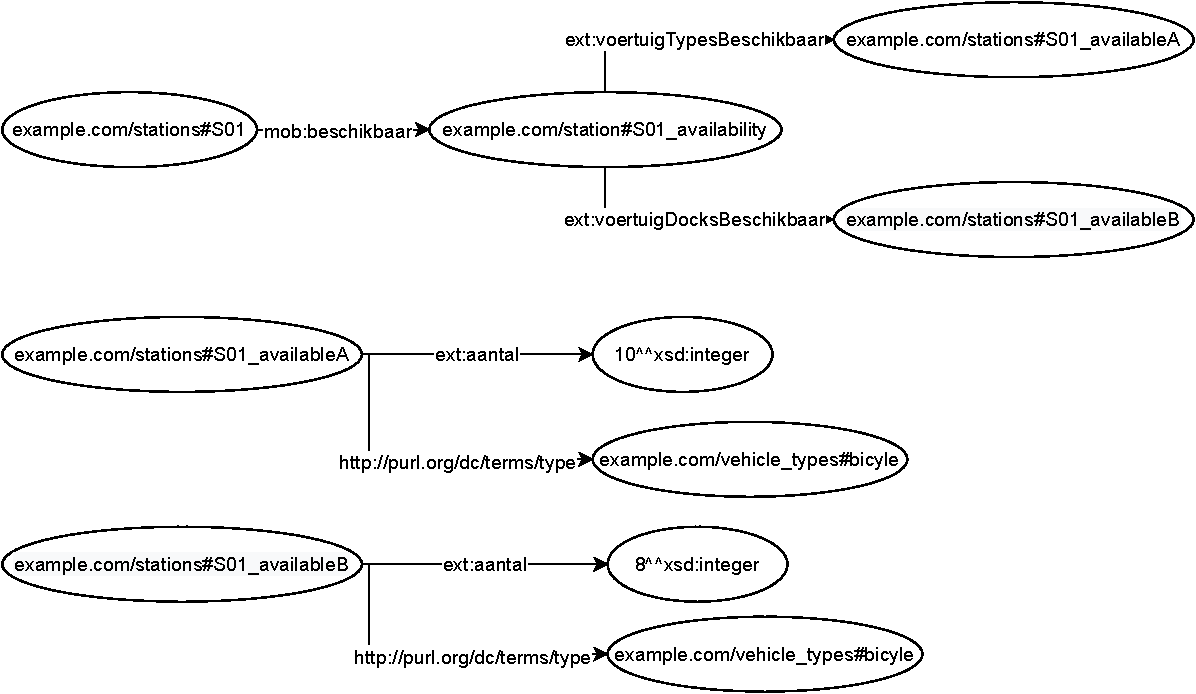
\includegraphics[width=\textwidth]{images/rdf_dataset.pdf}
		}
	\end{subfigure}
	\caption{Gegevensset gebruikmakend van RDF-model}
	\label{fig:rdf_gegevensset_voorbeeld}
\end{figure}
\chapter{Gegevens on-boarding}
\label{chap:on-boarding}

Uit een gesprek met Stijn Vernaillen, MaaS expert en bezig met gegevens rond mobiliteit bij stad Antwerpen, blijkt dat het moeilijk is een gegevensmodel en -formaat te verplichten aan \glspl{mobop}. 
Alhoewel het ideaal zou zijn mochten eigenaren van gegevens zelf hun gegevens in het gepaste RDF-model publiceren, zouden volgens hem niet alle operatoren over voldoende middelen beschikken om te kunnen investeren in het herpubliceren van hun gegevens in een door de overheid verplicht gegevensmodel\cite{vernaillen}.
Daarnaast is het niet de bedoeling operatoren extra te belasten met mijn doel hun gegevens in de OSLO-pijplijn te krijgen. In tegendeel: de oplossing moet de data-publisher zoveel mogelijk ontlasten.
In dit hoofdstuk worden methodes beschreven die aantonen dat het omvormen van hun gegevens om OSLO-conform te zijn maar een kleine inspanning vragen. Daarnaast kunnen ze worden begeleid door de OSLO-experten die OSLO-services (~\ref{sec:oslo_services}) aanbieden.
In volgende secties zullen gegevenssets gepubliceerd met het GBFS en NGSI model gebruikt worden aangezien dit populaire specificaties zijn bij fietsdeeloperatoren.

Om gegevens rond \glspl{mobop} te linken met andere gegevens in Vlaanderen, werd de OSLO mobiliteit: trips \& aanbod ontologie uitgebreid (hoofdstuk ~\ref{chap:ontologie_voor_fietsdeeloperatoren}). Eens gegevens gepubliceerd worden conform die OSLO-uitbreiding, zit het in de OSLO-pijplijn. Deze pijplijn kan toegang bieden tot allerhande services die verdere bewerkingen uitvoeren op gegevens: archivering, bewaren en ophalen van historische gegevens, ... De pijplijn en eraan gekoppelde services zijn nog volop in ontwikkeling. Eens ze beschikbaar zijn, zijn ook de gegevens klaar om er gebruik van te maken. Deze scriptie en specifiek deze sectie beschrijft deze on-boarding: het mappen van niet OSLO-conforme gegevens naar het wel OSLO-conform zijn.

\section{RML.io}
\label{sec:rml}
JSON is een populair formaat voor het bewaren en versturen van gegevens. Het wordt meestal gebruikt als formaat om gegevens, opgevraagd via een API, terug te geven. Veel gebruikte gegevensmodellen om gegevens rond fietsdeeloperatoren te publiceren in JSON zijn GBFS en NGSI. GBFS werd reeds omschreven in sectie~\ref{sec:GBFS}. Voorbeelden zijn de velo.json (bijlage A) dat gebruikmaakt van NGSI. En donkey.json (bijlage B) dat gebruikmaakt van GBFS. 
Een eerste use case om van deze gegevens Linked Data te genereren is door middel van de RML toolchain\footnote{\url{https://rml.io/}}. De eerste stap is het opbouwen van RML regels als tussenstap voor het genereren van LD. RML kan met YARRRML gegenereerd worden. Het codevoorbeeld in bijlage C is een YARRRML document waarmee de velo.json gegevensset uit bijlage A naar RML kan worden geserialiseerd.
Daarna wordt door middel van een RMLMapper\footnote{\url{https://github.com/RMLio/rmlmapper-java}} uit de RML regels Linked Data gegenereerd\footnote{\url{https://github.com/stijnbrysbaert/mapper}}.

\section{JSON naar JSON-LD}
\label{sec:json2jsonld}
Als tweede use case kan een JSON gegevensset omgevormd worden naar een JSON-LD formaat. JSON-LD brengt de mogelijkheid naar JSON om objecten aan elkaar te linken en te refereren naar andere objecten buiten het document met behulp van uri's (sectie ~\ref{sec:ngsi-ld}).
Het @context-sleutelwoord die dat mogelijk maakt krijgt een object mee dat er op verschillende manieren kan uit zien. Om te beginnen kunnen de sleutels van het JSON-object gemapt worden op voorlopige uri's die niet derefereerbaar zijn met een HTTP cliënt, verder in deze tekst dummy-URI's genoemd. Zo kan bijvoorbeeld de dummy URI \url{http://example.org/rdf#} als prefix worden gebruikt zoals in voorbeeld 1 (\ref{subsec:vb1}). Dit zorgt natuurlijk niet voor interoperabiliteit met andere gegevenssets, maar het geeft een idee van hoe de @context werkt.
Als tweede stap is het mogelijk om bij simpele RDF-modellen de uri's te gebruiken van dat RDF-model. Met simpel wordt hier bedoeld dat een instantie van een RDF-klasse enkel relaties heeft met een literal. Het predicaat in de RDF-triplet is dus van het RDF-type `owl:DatatypeProperty'. Wanneer er instanties zijn die referenties hebben naar andere instanties van klasses, wordt het moeilijk dit zonder meer dan met een @context op te lossen.

\subsection{JSON-object aanpassen}
Enerzijds kan de context worden toegevoegd aan het root-object van de gegevensset.
Wanneer de JSON bestaat uit één enkel object, kan de @context als extra object worden toegevoegd. Wanneer het om een array van objecten gaat, moeten die nodes gegroepeerd worden door middel van het `@included'-keyword. De array van objecten wordt toegevoegd aan een root-object, waartoe ook de @context behoort, met de sleutel @included.

\subsection{HTTP Link Header}
Anderzijds kan er in de response headers van de gegevens-endpoint een referentie meegegeven worden die leidt naar de JSON-LD context. Dit gebeurt door een HTTP Link header toe te voegen aan de response headers waarin gerefereerd wordt naar de juiste JSON-LD context.
Op deze manier wordt de JSON machine-interpreteerbaar zonder dat ontwikkelaars hun gegevenssets moeten aanpassen~\cite{JSON-LD1.1}.
De syntaxt van de HTTP Link header is de volgende~\cite{httplinkheader}:
\begin{code}
\begin{minted}[breaklines]{json}
Link: < uri-reference >; param1="value1"; param2="value2"
\end{minted}
\end{code}
De \textit{uri-reference} moet worden vervangen door een referentie naar het JSON-document met daarin de JSON-LD context. Er zijn twee parameters verplicht: \textit{rel="http://www.w3.org/ns/json-ld\#context"} en \textit{type="application/ld+json"} die vaste waarden hebben. 

Om bijvoorbeeld bijlage A of B te kunnen gebruiken als gegevensbron bij een SPARQL engine kan de Link Header in Listing~\ref{code:link_header} worden gebruikt. Hier wordt als voorbeeld de URI \url{https://example.org/context.jsonld} gebruikt, deze moet in een echt scenario vervangen worden door een HTTP URI de refereert naar een JSON-LD context zoals in Listing~\ref{code:context}.
\begin{code}
\begin{minted}[breaklines]{json}
"Link": '<https://example.org/context.jsonld>; rel="http://www.w3.org/ns/json-ld#context"; type="application/ld+json"'
\end{minted}
\caption{HTTP Link header}
\label{code:link_header}
\end{code}

\subsection{Voorbeeld 1}
\label{subsec:vb1}
De @context in codevoorbeeld~\ref{code:context} kan worden gebruikt om het JSON-object in bijlage E te transformeren naar JSON-LD. Het is belangrijk de objecten met sleutels `id' en `type' toe te voegen aan de context om het geheel te laten werken. Het mapt de betreffende sleutels op de JSON-LD sleutelwoorden `@id' en `@type'. Op die manier zullen de sleutels worden geïnterpreteerd als respectievelijk het subject en het rdf:type object van de gegevensset.

\begin{code}
\begin{minted}[breaklines]{json}
{
    "@context": [
        {
            "ext": "https://stijnbrysbaert.github.io/OSLO-extension/vocabulary.ttl#"
        },
        {
            "example": "http://www.example.org/rdf#"
        },
        {
            "availableBikeNumber": {
                "@id": "example:availableBikeNumber"
            }
        },
        {
            "freeSlotNumber": {
                "@id": "example:freeSlotNumber"
            }
        },
        {
            "BikeHireDockingStation": {
                "@id": "ext:Station"
            }
        },
        {
            "id": "@id"
        },
        {
            "type": "@type"
        }
    ]
}
\end{minted}
\caption{@context met dummy en werkelijke uri's}
\label{code:context}
\end{code}

In deze context wordt als voorbeeld de sleutel `BikeHireDockingStation' gemapt op ext:Station. Hiermee wordt aangetoond dat het mogelijk is ook uri's van eigen RDF-modellen te mappen op de sleutels van objecten. Simpele gegevenssets kunnen zo met enkel en alleen een @context gemapt worden naar een simpel RDF-model. 

\subsection{Voorbeeld 2}
\label{subsec:vb2}
Om de JSON in bijlage D naar JSON-LD te transformeren is een extra @context nodig bovenop de context in \ref{code:context}. Deze JSON gegevensset maakt gebruik van een van de gegevensmodellen van de NGSI specificatie (Bike Hire Docking Station) en werd gepubliceerd in genormaliseerde vorm (\ref{sec:ngsi-ld}). Daarom is het belangrijk om de externe context \url{https://uri.etsi.org/ngsi-ld/v1/ngsi-ld-core-context.jsonld} toe te voegen. Deze zal de sub-eigenschappen mappen op een URI zodat ze te queryen zijn. Zo zal bijvoorbeeld de sub-eigenschap `value' gemapt worden op URI \url{https://uri.etsi.org/ngsi-ld/hasValue}.
Om problemen te vermijden bij het overschrijven van uri's die zijn opgenomen in de ngsi-ld core context, zet je deze context best bovenaan in het context-object.

Gezien het NGSI gegevensmodel zal een CONSTRUCT-query nodig zijn om de sub-eigenschappen weg te werken. Deze CONSTRUCT-query zal RDF-triples genereren met de nodes die het in de WHERE-clausule van de SPARQL query uit de gegevensbron haalt. Het resultaat is een gegevensset gemapt naar het gewenste RDF-model, in dit voorbeeld de uitbreiding op OSLO mobiliteit: trips \& aanbod. 

\begin{code}
\begin{minted}[breaklines]{sparql}
PREFIX dct: <http://purl.org/dc/terms/>
PREFIX example: <http://www.example.org/rdf#>
PREFIX ext: <https://stijnbrysbaert.github.io/OSLO-extension/vocabulary.ttl#>
PREFIX ngsild: <https://uri.etsi.org/ngsi-ld/>
PREFIX trips: <https://data.vlaanderen.be/ns/mobiliteit/trips-en-aanbod#>

CONSTRUCT{
    ?s a ext:Station .
    ?s trips:Transportobject.beschikbaarheid _:b .
    _:b ext:voertuigTypesBeschikbaar _:items .
    _:items a ext:VoertuigenBeschikbaar .
    _:items ext:aantal ?aantal_bike .
    _:b ext:voertuigDocksBeschikbaar _:docks .
    _:docks a ext:DocksBeschikbaar .
    _:docks ext:aantal ?aantal_slot .
    _:items dct:type _:type .
    _:type a trips:Resourcetype .
    _:docks dct:type _:type .
}
WHERE {
    ?s a ext:Station .
    ?s example:availableBikeNumber ?obj_abn .
    ?obj_abn ngsild:hasValue ?aantal_bike .
    ?s example:freeSlotNumber ?obj_slot .
    ?obj_slot ngsild:hasValue ?aantal_slot .
}
\end{minted}
\caption{SPARQL query met CONSTRUCT-clausule}
\label{code:construct}
\end{code}

In voorbeelden 1 en 2 werd bewust de `location'-eigenschap buiten beschouwing gelaten. Doordat de NGSI specificatie coördinaten in hun model implementeert aan de hand van GeoJSON is het niet mogelijk om met een SPARQL query individuele waarden te mappen op een specifieke URI. Dit komt doordat GeoJSON coördinaten bijhoudt in een array, terwijl het niet mogelijk is met een SPARQL query elementen uit een array te selecteren op basis van hun index. JSON-LD 1.1\footnote{\url{https://www.w3.org/TR/json-ld11/}} lost dit deels op met GeoJSON-LD\footnote{\url{https://geojson.org/geojson-ld/}}.
Een andere oplossing hiervoor is gebruikmaken van de RML.io toolchain uit sectie \ref{sec:rml} dat wel overweg kan met arrays en hun indexen.

\subsection{Voorbeeld 3}
\label{subsec:vb3}
In voorbeelden 1 en 2 werd telkens een gegevensset volgens het NGSI model gebruikt. In dit voorbeeld is het de beurt aan de GBFS specificatie met een gegevensset uit bijlage A: donkey.json. Om op deze set een SPARQL query te kunnen uitvoeren moet er opnieuw een @context worden toegevoegd zodat de JSON getransformeerd wordt naar JSON-LD. 
Deze keer voegen we aan de @context het `@vocab'-sleutelwoord toe. Dit sleutelwoord zorgt er voor dat er een default vocabularium aan de context wordt toegevoegd. Alle eigenschappen en types, waarvoor geen andere URI in de context werd gespecificeerd, zullen dezelfde prefix krijgen.
De sleutels in de JSON worden allen gemapt op een default URI met de prefix die werd meegegeven aan het @vocab-sleutelwoord, aangevuld met hun oorspronkelijke sleutel. Zonder meer kan deze JSON-LD nu worden gequeryd met volgende SPARQL query.

\begin{code}
\centering
\begin{minted}[breaklines]{sparql}
PREFIX default: <http://example.org/rdf#>

SELECT ?s ?id ?items ?docks WHERE {
    ?s default:fields ?fields .
    ?fields default:station_id ?id .
    ?fields default:num_bikes_available ?items .
    ?fields default:num_docks_available ?docks .
}
\end{minted}
\caption{SPARQL met NGSI-LD default context}
\label{ngsild-default-context}
\end{code}

Opnieuw kan er met een aanvullende CONSTRUCT-clausule een gegevensset geconstrueerd worden volgens het gewenste RDF-model.

\section{De mogelijkheden opgelijst}
Met de RML.io toolchain kunnen vanuit verschillende gegevensformaten (CSV, JSON, XML) RML regels gegenereerd worden. In een tweede stap wordt met behulp van die RML regels Linked Data gegenereerd. In het YARRRML document kunnen functies worden toegevoegd aan subject, predicaten en objecten die de gegevens kunnen manipuleren voordat het naar een LD gegevensset gemapt wordt. In bijlage C - velo.yaml wordt er zo een functie gebruikt.

Een simpelere manier, maar met beperktere mogelijkheid wegens het gebrek aan functies, is JSON-LD. Iedere JSON gegevensbron kan relatief gemakkelijk worden getransformeerd naar JSON-LD waardoor het te queryen is met SPARQL queries. In de @context kunnen de sleutels uit de JSON-objecten gemapt worden op URI's. De context kan op verschillende manieren met verschillende doeleinden worden opgebouwd door gebruik te maken van:

\begin{itemize}
    \item \textbf{default URI's} met behulp van het @vocab-sleutelwoord die daarna naar een definitief RDF-model geconstrueerd worden met een CONSTRUCT-query
    \item \textbf{RDF-model URI's} zodat het direct te publiceren is als LD gegevensset
    \item \textbf{NGSI-LD core context} wanneer een NGSI gegevensmodel wordt gebruikt. Deze context mapt de meta-gegevens van de object-eigenschappen naar gepaste uri's die daarna door middel van een CONSTRUCT-query naar het gewenste RDF-model kunnen worden gemapt
\end{itemize}

Afhankelijk van het formaat van de aangeleverde gegevensset en de eventuele manipulaties die er op moeten gebeuren is het tranformeren naar JSON-LD een snellere manier om de stap naar Linked Data te maken dan het gebruik van RML.
\chapter{Conclusie}
\label{chap:conclusie}
Het OSLO programma van de Vlaamse overheid biedt RDF vocabularia waarin gegevens worden gemodelleerd en gepubliceerd als Linked Open Data. Dit zorgt voor interoperabiliteit tussen de gegevens van honderden publieke sector diensten. Geld en tijd worden bespaard doordat de diensten gegevens kunnen uitwisselen tussen elkaar gebruikmakend van hun eigen business proces en ICT systemen.
OSLO mobiliteit: trips \& aanbod is één van die OSLO vocabularia. Dit vocabularium focust zich op personen die reizen en de mobiliteitsdiensten die ze daarvoor ter beschikking hebben. In hoofdstuk~\ref{chap:ontologie_voor_fietsdeeloperatoren} werd voor dit vocabularium een uitbreiding gemaakt zodat ook fietsdeeloperatoren hun gegevens in dit model kunnen publiceren. Dankzij de abstracte implementatie, geleend uit de GBFS specificatie, kunnen ook andere types vervoersmiddelen in de deeleconomie hun gegevens modelleren met dit vocabularium.

Aangezien operatoren moeilijk te overtuigen zijn hun gegevens direct te publiceren in een door de overheid verplicht gegevensmodel, moeten er tools worden voorzien die de gegevens mappen. Na het mappen dienen gegevens te worden herpubliceerd  als Linked Open Data. Dat mappen kan op een paar verschillende manieren beschreven in hoofstuk~\ref{chap:on-boarding}. De meeste gegevenssets van fietsdeeloperatoren worden gepubliceerd in een JSON-formaat gemodelleerd volgens de GBFS of NGSI specificatie. Door de gegevens te transformeren naar JSON-LD is ze sneller te herpubliceren als LOD dan met de RML-methode. Om via de RML-toolchain naar LD te mappen, moet er eerst een YARRRML document geschreven worden die RML-regels genereert. De snelste manier om te transformeren naar JSON-LD is door een default vocabularium toe te voegen aan de context met het @vocab-sleutelwoord. Er moeten dan geen extra URIs per term worden gedefinieerd. Met een SPARQL query met CONSTRUCT-clausule kan dan een Linked Data gegevensset geconstrueerd worden met het gewenste RDF-model. Wanneer het oorspronkelijke gegevensformaat geen JSON is, zal er toch moeten worden teruggegrepen naar de RML-toolchain.

Deze stappen maken deel uit van het on-boardingsproces van gegevens naar de pijplijn van Vlaamse, OSLO conforme, gegevens. Eens de gegevens in deze pijplijn zitten, kunnen ze geconsumeerd, gemanipuleerd voor andere doeleinden en gearchiveerd worden. Zo moet er geen geld meer besteed worden aan diensten die de gegevens laten werken, maar zullen de gegevens werken voor efficiëntere diensten.
\bibliography{referenties}

\begin{appendices}
\section*{Bijlage A - donkey.json}
\label{app:donkey.json}
Snipit van een Donkey Republic gegevensset in JSON-formaat gehaald uit de open database van stad Gent\footnote{\url{https://data.stad.gent/explore/dataset/donkey-republic-beschikbaarheid-deelfietsen-per-station}}. Deze array bevat twee objecten die elk informatie over de status van dat station bijhouden.
\begin{code}
\begin{minted}[breaklines]{json}
[
    {
        "datasetid": "donkey-republic-beschikbaarheid-deelfietsen-per-station",
        "recordid": "62d9aa911167ba3f491f93f7ce7adfb530925c8f",
        "fields": {
            "last_reported": "1600650631",
            "num_docks_available": 2,
            "is_renting": 1,
            "station_id": "12419",
            "is_installed": 1,
            "num_bikes_available": 1,
            "is_returning": 1
        },
        "record_timestamp": "2020-12-21T19:30:03.126+01:00"
    },
    {
        "datasetid": "donkey-republic-beschikbaarheid-deelfietsen-per-station",
        "recordid": "fbbd057f9b0f507a7bd9b6200c3a71e2a12bbc97",
        "fields": {
            "last_reported": "1607735889",
            "num_docks_available": 0,
            "is_renting": 1,
            "station_id": "16619",
            "is_installed": 1,
            "num_bikes_available": 3,
            "is_returning": 1
        },
        "record_timestamp": "2020-12-21T19:30:03.126+01:00"
    }
]
\end{minted}
\end{code}

\section*{Bijlage B - velo.json}
\label{app:velo.json}
Snipit van een gegevensset met Antwerpse Velo's, in JSON-formaat gehaald uit de 
\begin{code}
\begin{minted}[breaklines]{json}
[
    {
        "id": "BikeHireDockingStation:Antwerpen:035",
        "type": "BikeHireDockingStation",
        "address": {
            "type": "PostalAddress",
            "value": {
                "streetAddress": "cockerillkaai",
                "postalCode": "2000",
                "addressCountry": "BE"
            },
            "metadata": {}
        },
        "areaServed": {
            "type": "Text",
            "value": "Antwerpen",
            "metadata": {}
        },
        "availableBikeNumber": {
            "type": "Number",
            "value": 8,
            "metadata": {
                "timestamp": {
                    "type": "DateTime",
                    "value": "2020-12-22T08:32:12.00Z"
                }
            }
        },
        "freeSlotNumber": {
            "type": "Number",
            "value": 28,
            "metadata": {
                "timestamp": {
                    "type": "DateTime",
                    "value": "2020-12-22T08:32:12.00Z"
                }
            }
        },
        "location": {
            "type": "geo:json",
            "value": {
                "type": "Point",
                "coordinates": [
                    4.3877,
                    51.210318
                ]
            },
            "metadata": {}
        }
]
\end{minted}
\end{code}

\section*{Bijlage C - velo.yaml}
\label{app:velo.yaml}

\begin{code}
\begin{minted}[breaklines]{yaml}
prefixes:
  ex: 'https://example.be#'
  adr:  'https://data.vlaanderen.be/ns/adres#'
  dienst: 'https://stijnbrysbaert.github.io/OSLO-extension/mobiliteitsdiensten.ttl#'
  dc:   'http://purl.org/dc/terms/'
  ext:  'https://stijnbrysbaert.github.io/OSLO-extension/vocabulary.ttl#'
  foaf: 'http://xmlns.com/foaf/0.1/'
  geo:  'http://www.w3.org/2003/01/geo/wgs84_pos#'
  geonames: 'http://www.geonames.org/ontology#'
  grel: 'http://users.ugent.be/~bjdmeest/function/grel.ttl#'
  idlab-fn: 'http://example.com/idlab/function/'
  locn: 'http://www.w3.org/ns/locn#'
  mv:   'http://schema.mobivoc.org/'
  prov: 'http://www.w3.org/ns/prov#'
  rdf:  'http://www.w3.org/1999/02/22-rdf-syntax-ns#'
  rdfs: 'http://www.w3.org/2000/01/rdf-schema#'
  tn:   'https://data.vlaanderen.be/ns/transportnetwerk#'
  trips: 'https://data.vlaanderen.be/ns/mobiliteit/trips-en-aanbod#'
  xsd:  'http://www.w3.org/2001/XMLSchema#'

mappings:
  station:
    sources:
      - ['velo.json~jsonpath', '$.velos[*]']
    s: ex:$(id)
    po:
      - [a, [ext:Station, dc:Location]]
      - [rdfs:label, $(name.value)]
      - p: locn:geometry
        o:
          mapping: location
          condition:
            function: equal
            parameters:
              - [str1, $(id)]
              - [str2, $(id)]
      - p: 'trips:Transportobject.beschikbaarheid'
        o: 
          mapping: status
          condition:
            function: equal
            parameters:
              - [str1, $(id)]
              - [str2, $(id)]

  location:
    sources:
      - ['velo.json~jsonpath', '$.velos[*]']
    s: ex:location_$(id)
    po:
      - [a, geo:Point]
      - [geo:long, '$(location.value.coordinates[0])']
      - [geo:lat, '$(location.value.coordinates[1])']

  voertuigenBeschikbaar:
    sources:
      - ['velo.json~jsonpath', '$.velos[*]']
    s: ex:itemsAvailable_$(id)
    po:
      - [a, ext:VoertuigenBeschikbaar]
      - [ext:aantal, $(availableBikeNumber.value)]
      
  docksBeschikbaar:
    sources:
      - ['velo.json~jsonpath', '$.velos[*]']
    s: ex:docksAvailable_$(id)
    po:
      - [a, ext:DocksBeschikbaar]
      - [ext:aantal, $(freeSlotNumber.value)]

  status:
    sources:
      - ['velo.json~jsonpath', '$.velos[*]']
    s: ex:status_$(id)
    po:
      - [a, trips:Beschikbaarheid]
      - p: ext:voertuigTypesBeschikbaar
        o:
          mapping: voertuigenBeschikbaar
          condition:
            function: equal
            parameters:
              - [str1, $(id)]
              - [str2, $(id)]
      - p: ext:voertuigDocksBeschikbaar
        o:
          mapping: docksBeschikbaar
          condition:
            function: equal
            parameters:
              - [str1, $(id)]
              - [str2, $(id)]
      - [prov:generatedAtTime, $(availableBikeNumber.metadata.timestamp.value)]
      - p: ext:actief
        o:
          value: "true"
          datatype: "xsd:boolean"
        condition:
          function: idlab-fn:equal
          parameters:
            - [grel:valueParameter, $(status.value)]
            - [grel:valueParameter2, "working"]
      - p: ext:actief
        o:
          value: "false"
          datatype: "xsd:boolean"
        condition:
          function: idlab-fn:notEqual
          parameters:
            - [grel:valueParameter, $(status.value)]
            - [grel:valueParameter2, "working"]
\end{minted}
\end{code}

\section*{Bijlage D - NGSI normalized}
Genormaliseerd voorbeeld van een NGSI resultaat\footnote{\url{https://fiware-datamodels.readthedocs.io/en/latest/Transportation/Bike/BikeHireDockingStation/doc/spec/index.html}}.
\begin{code}
\begin{minted}[breaklines]{json}
{
    "id": "Bcn-BikeHireDockingStation-1",
    "type": "BikeHireDockingStation",
    "status": {
        "value": "working"
    },
    "availableBikeNumber": {
        "value": 20,
        "metadata": {
            "timestamp": {
                "type": "DateTime",
                "value": "2018-09-25T12:00:00"
            }
        }
    },
    "freeSlotNumber": {
        "value": 10
    },
    "location": {
        "type": "geo:json",
        "value": {
            "type": "Point",
            "coordinates": [2.180042, 41.397952]
        }
    },
    "address": {
        "type": "PostalAddress",
        "value": {
            "addressCountry": "ES",
            "addressLocality": "Barcelona",
            "streetAddress": "Gran Via Corts Catalanes,760"
        }
    }
}

\end{minted}
\end{code}

\section*{Bijlage E - NGSI key-value paren}
Een versimpelde weergave van een NGSI resultaat\footnote{\url{https://fiware-datamodels.readthedocs.io/en/latest/Transportation/Bike/BikeHireDockingStation/doc/spec/index.html}}, meestal gebruikt voor consumers en daarom zeer handig in gebruik voor de use cases in deze scriptie.
\begin{code}
\begin{minted}[breaklines]{json}
{
    "id": "malaga-bici-7",
    "type": "BikeHireDockingStation",
    "name": "07-Diputacion",
    "location": {
        "coordinates": [-4.43573, 36.699694],
        "type": "Point"
    },
    "availableBikeNumber": 18,
    "freeSlotNumber": 10,
    "address": {
        "streetAddress": "Paseo Antonio Banderas (Diputación)",
        "addressLocality": "Malaga",
        "addressCountry": "España"
    },
    "description": "Punto de alquiler de bicicletas próximo a Diputación",
    "dateModified": "2017-05-09T09:25:55.00Z"
}
\end{minted}
\end{code}

\end{appendices}

\end{document}
